% 
% exemplo genérico de uso da classe iiufrgs.cls
% $Id: iiufrgs.tex,v 1.1.1.1 2005/01/18 23:54:42 avila Exp $
% 
% This is an example file and is hereby explicitly put in the
% public domain.
% 
\documentclass[cic,tc]{iiufrgs}
% Para usar o modelo, deve-se informar o programa e o tipo de documento.
% Programas :
% * cic       -- Graduação em Ciência da Computação
% * ecp       -- Graduação em Ciência da Computação
% * ppgc      -- Programa de Pós Graduação em Computação
% * pgmigro   -- Programa de Pós Graduação em Microeletrônica
% 
% Tipos de Documento:
% * tc                -- Trabalhos de Conclusão (apenas cic e ecp)
% * diss ou mestrado  -- Dissertações de Mestrado (ppgc e pgmicro)
% * tese ou doutorado -- Teses de Doutorado (ppgc e pgmicro)
% * ti                -- Trabalho Individual (ppgc e pgmicro)
% 
% Outras Opções:
% * english    -- para textos em inglês
% * openright  -- Força início de capítulos em páginas ímpares (padrão da
% biblioteca)
% * oneside    -- Desliga frente-e-verso
% * nominatalocal -- Lê os dados da nominata do arquivo nominatalocal.def

% === PACKAGES ===
% Use unicode
\usepackage[utf8]{inputenc}   % pacote para acentuação
% Necessário para incluir figuras
\usepackage{graphicx}         % pacote para importar figuras
\usepackage{times}            % pacote para usar fonte Adobe Times
% \usepackage{palatino}
% \usepackage{mathptmx}       % p/ usar fonte Adobe Times nas fórmulas
\usepackage[alf,abnt-emphasize=bf, abnt-etal-list=0, abnt-etal-cite=2]{abntex2cite}	% pacote para usar citações abnt
\usepackage{verbatim}
\usepackage{amsmath}
\usepackage{algorithm}
\usepackage[noend]{algpseudocode}
\usepackage{color, colortbl}
\usepackage{placeins}
\usepackage{chngpage}
\usepackage{hyperref}
\usepackage{rotating}
\usepackage{graphics}
\usepackage{array}

% === DEFINITIONS === 
\floatname{algorithm}{Algoritmo}
\graphicspath{ {./figuras/} }
\renewcommand{\arraystretch}{1.5}
\definecolor{darkorange}{rgb}{0.9647058823529412, 0.6980392156862745, 0.4196078431372549}
\definecolor{lightorange}{rgb}{0.9768, 0.79608, 0.61176}
\newcolumntype{o}{>{\columncolor{lightorange}}r}
\newcolumntype{P}[1]{>{\centering\arraybackslash}p{#1}}

% comandos miraculosos para evitar quebra de palavras
\tolerance=1
\emergencystretch=\maxdimen
\hyphenpenalty=10000
\hbadness=10000


% 
% Informações gerais
% 
\title{Portal de Vagas - implementação de uma ferramenta para divulgação de bolsas e estágios a alunos}

\author{Flesch}{Jean Ampos}
% alguns documentos podem ter varios autores:
% \author{Flaumann}{Frida Gutenberg}
% \author{Flaumann}{Klaus Gutenberg}

% orientador e co-orientador são opcionais (não diga isso pra eles :))

\advisor[Profa.~Dra.]{Galante}{Renata}
% \coadvisor[Prof.~Dr.]{Knuth}{Donald Ervin}

% a data deve ser a da defesa; se nao especificada, são gerados
% mes e ano correntes
% \date{maio}{2001}

% o local de realização do trabalho pode ser especificado (ex. para TCs)
% com o comando \location:
% \location{Itaquaquecetuba}{SP}

% itens individuais da nominata podem ser redefinidos com os comandos
% abaixo:
% \renewcommand{\nominataReit}{Prof\textsuperscript{a}.~Wrana Maria Panizzi}
% \renewcommand{\nominataReitname}{Reitora}
% \renewcommand{\nominataPRE}{Prof.~Jos{\'e} Carlos Ferraz Hennemann}
% \renewcommand{\nominataPREname}{Pró-Reitor de Graduação}
\renewcommand{\nominataPRAPG}{Prof.~Vladimir Pinheiro do Nascimento}
\renewcommand{\nominataPRAPGname}{Pró-Reitor de Graduação}
% \renewcommand{\nominataDir}{Prof.~Philippe Olivier Alexandre Navaux}
% \renewcommand{\nominataDirname}{Diretor do Instituto de Inform{\'a}tica}
\renewcommand{\nominataCoord}{Prof.~Sérgio Luis Cechin}
\renewcommand{\nominataCoordname}{Coordenador do Curso de Ciência de Computação}
% \renewcommand{\nominataBibchefe}{Beatriz Regina Bastos Haro}
% \renewcommand{\nominataBibchefename}{Bibliotec{\'a}ria-chefe do Instituto de Inform{\'a}tica}
% \renewcommand{\nominataChefeINA}{Prof.~Jos{\'e} Valdeni de Lima}
% \renewcommand{\nominataChefeINAname}{Chefe do \deptINA}
% \renewcommand{\nominataChefeINT}{Prof.~Leila Ribeiro}
% \renewcommand{\nominataChefeINTname}{Chefe do \deptINT}

% A seguir são apresentados comandos específicos para alguns
% tipos de documentos.

% Relatório de Pesquisa [rp]:
% \rp{123}             % numero do rp
% \financ{CNPq, CAPES} % orgaos financiadores

% Trabalho Individual [ti]:
% \ti{123}     % numero do TI
% \ti[II]{456} % no caso de ser o segundo TI

% Monografias de Especialização [espec]:
% \espec{Redes e Sistemas Distribuídos}      % nome do curso
% \coord[Profa.~Dra.]{Weber}{Taisy da Silva} % coordenador do curso
% \dept{INA}                                 % departamento relacionado

% 
% palavras-chave
% iniciar todas com letras minúsculas, exceto no caso de abreviaturas
% 
\keyword{Detecção de Anomalias}
\keyword{Dados de Sensores}
\keyword{Redes de Sensores Sem Fio}
\keyword{\textit{Big Data}}

%\settowidth{\seclen}{1.10~}

% 
% inicio do documento
% 
\begin{document}

% folha de rosto
% às vezes é necessário redefinir algum comando logo antes de produzir
% a folha de rosto:
% \renewcommand{\coordname}{Coordenadora do Curso}
\maketitle

% dedicatoria
%\clearpage
%\begin{flushright}
%     \mbox{}\vfill
%     {\sffamily\itshape
%       ``If I have seen farther than others,\\
%       it is because I stood on the shoulders of giants.''\\}
%     --- \textsc{Sir~Isaac Newton}
%\end{flushright}

% agradecimentos
\chapter*{Agradecimentos}
É com muita felicidade que eu encerro minha jornada pelo curso de graduação em Ciência da Computação. Concluo o curso com a certeza de que obtive muitas conquistas, mas que ainda há muito a aprender. Aproveito esta oportunidade para agradecer a todos que me apoiaram, eu não teria conseguido sem vocês.

Agradeço aos meus pais, Luiz Fernando Gonzaga e Marli dos Santos Gonzaga, e aos meus irmãos, Gabriel e Samara dos Santos Gonzaga, por serem meu maior suporte. Obrigado por serem o porto para o qual eu sempre posso voltar. Agradeço a minha namorada, Victória Isoppo, por sempre me incentivar e acreditar em mim. Obrigado por todo o apoio que me deste.~Agradeço a todos os meus amigos, principalmente os que de alguma forma me ajudaram durante o desenvolvimento desse trabalho. Me desculpem pelas dezenas de convites recusados.~Agradeço a minha orientadora, Dr.ª Renata Galante, que sempre esteve disponível a qualquer momento para me guiar, dar sugestões e me tranquilizar durante o desenvolvimento deste trabalho. Finalmente, obrigado a todos os professores e funcionários do Instituto de Informática que participaram de alguma forma da minha jornada.

Sou infinitamente grato.



% resumo na língua do documento
\begin{abstract}
	Apesar de serem uma solução de monitoramento barata, devido a restrições de processamento, comunicação e energia, redes de sensores estão sujeitas a leituras corrompidas e anômalas. Neste trabalho, o \textit{framework} para a detecção de anomalias proposto por \cite{MasterMichaels2014} foi implementado e avaliado. Foram propostas mudanças em duas etapas do algoritmo e mediu-se o seu impacto no desempenho. O \textit{framework} implementado foi avaliado em dois conjuntos de dados de redes de sensores sem fio com resultados satisfatórios, detectando 80\% das anomalias presentes. Das duas mudanças propostas, apenas uma resultou em uma leve melhoria da capacidade de detecção do \textit{framework}. Este trabalho fornece uma análise detalhada dos componentes do \textit{framework}, o que pode ser tomado como base para futuras melhorias.
\end{abstract}

% resumo na outra língua
% como parametros devem ser passados o titulo e as palavras-chave
% na outra língua, separadas por vírgulas
\begin{englishabstract}{
Implementation of a Framework for Contextual Anomaly Detection in Sensor Data}{Anomaly Detection.  Sensor Data. Wireless Sensor Networks. Big Data}
	Despite being a low cost solution for the monitoring problem, due to processing, communication and energy constraints, wireless sensor networks are subject to corrupt and anomalous readings. In this work, the anomaly detection framework proposed by \cite{MasterMichaels2014} has been implemented and evaluated. Changes in two steps of the algorithm were suggested and their impact on the performance was measured. The implemented framework was analyzed on two wireless sensor networks data sets with good results, detecting 80\% of the present anomalies. Of the two proposed changes, only one resulted in a slight improvement in the \textit{framework's} detection capacity. This work provides a detailed analysis of the framework's components, that can be a basis for future improvements.
\end{englishabstract}

% lista de figuras
\listoffigures

% lista de tabelas
\listoftables

% lista de abreviaturas e siglas
% o parametro deve ser a abreviatura mais longa
\begin{listofabbrv}{SPMD}
    \item[RB] Rede Bayesiana
    \item[FDCA] Framework para a Detecção Contextual de Anomalias
    \item[VP] Verdadeiros Positivos
    \item[VN] Verdadeiros Negativos
    \item[FP] Falsos Positivos
    \item[FN] Falsos Negativos
\end{listofabbrv}

% idem para a lista de símbolos
% \begin{listofsymbols}{$\alpha\beta\pi\omega$}
%     \item[$\sum{\frac{a}{b}}$] Somatório do produtório
%     \item[$\alpha\beta\pi\omega$] Fator de inconstância do resultado
% \end{listofsymbols}

% sumario
\tableofcontents

% ========== CAP 1 ==============
\chapter{Introdução}

Redes de sensores sem fio são uma solução flexível e de baixo custo para o monitoramento de processos industriais modernos. Porém, devido ao \textit{hardware} de baixo custo, interferência e ambientes hostis em que essas redes são implantadas, é comum que os sensores apresentem leituras corruptas ou faltantes \cite{wireless2002}. Outro aspecto importante é que, à medida que essas redes crescem em número de nodos, fica mais difícil processar o grande volume de dados e identificar anomalias. Anomalias, nesse contexto, podem indicar leituras corrompidas, que prejudicam a análise correta dos dados, ataques à rede de sensores ou eventos incomuns, que merecem atenção especial de um analista \cite{AnomalyDetectionSurvey2009}.

O problema de detecção de anomalias consiste em encontrar padrões ou eventos em um conjunto de dados que não correspondem a uma noção bem definida de normalidade. Essas anomalias podem ser de 3 tipos: pontuais, que são anômalas com respeito a todo o conjunto de dados; contextuais, que são anômalas apenas quando observadas em relação ao seu contexto; ou coletivas, que são valores que são anômalos apenas quando ocorrem em conjunto. Os algoritmos de detecção podem ser supervisionados, semi-supervisionados ou não-supervisionados. Um algoritmo de detecção de anomalias recebe como entrada um conjunto de dados e retorna uma lista de anotações classificando cada instância de dado como normal ou anômalo.

Vários trabalhos propõem soluções para o problema detecção de anomalias em redes de sensores. \cite{Ellipsoids2009} apresenta um método que realiza detecção de anomalias através do agrupamento de elipsoides. O trabalho não leva em consideração a informação de contexto dos dados. O método proposto por \cite{BayesianBelief} utiliza redes Bayesianas para a detecção de anomalias em redes de sensores, modelando na rede a informação de dependência entre os atributos. Essa informação de dependência deve ser determinada por um especialista humano. A Pontuação de Anomalia Baseada em Histograma \cite{hbos2012} pode ser utilizada na detecção de anomalias em dados de sensores, mas o algoritmo não consegue detectar anomalias locais.

O objetivo do presente trabalho é implementar o \textit{framework} de detecção de anomalias proposto por \citeauthor{ContextualMichael2014} no trabalho intitulado \textit{Contextual Anomaly Detection Framework for Big Sensor Data} (\citeyear{ContextualMichael2014}) e avaliar em conjuntos de dados do mundo real. O objetivo secundário é buscar pontos onde o \textit{framework} pode ser melhorado, propor mudanças e analisar o impacto dessas mudanças nos resultados. O sistema, denominado \textit{Framework para a Detecção Contextual de Anomalias} (FDCA), foi implementado em \textit{Python}, com a utilização das bibliotecas \textit{Scikit-learn}, \textit{Numpy} e \textit{Pandas}. O FDCA foi avaliado em dois conjuntos de dados de redes de sensores sem fio. Foram propostas e avaliadas mudanças em duas etapas do algoritmo.~O FDCA apresentou bons resultados para as avaliações, detectando 80\% das anomalias presentes nos dois conjuntos com menos de 2 milissegundos de avaliação por instância de dado. Das duas mudanças propostas, apenas uma resultou em uma leve melhoria da capacidade de detecção do \textit{framework}.~Este trabalho fornece uma análise detalhada dos componentes do \textit{framework}, o que pode ser tomado como base para futuras melhorias.

O restante deste trabalho segue a seguinte organização. O Capítulo~\ref{levantamento} apresenta a fundamentação teórica e trabalhos relacionados. O Capítulo~\ref{cap_baseline} descreve em detalhes o trabalho escolhido como base para este trabalho.~O Capítulo~\ref{implementacao} apresenta a implementação do trabalho descrito no Capítulo~\ref{cap_baseline}, discutindo decisões tomadas durante o desenvolvimento e apresenta duas propostas de mudanças no algoritmo. O Capítulo~\ref{experimentos} descreve os conjuntos de dados escolhidos para a avaliação do \textit{framework}, os experimentos realizados e apresenta os resultados obtidos. Finalmente, o Capítulo~\ref{conclusao} discute as conclusões e possíveis futuros trabalhos. O Apêndice~\ref{app_ibrl} contém exemplos de linhas do conjunto de dados \textit{IBRL}. O Apêndice~\ref{app_issnip} contém exemplos de linhas do conjunto de dados \textit{ISSNIP}.

% ========== CAP 2 ==============
\chapter{Levantamento Bibliográfico}
\label{levantamento}
Neste capítulo é apresentado o levantamento bibliográfico relacionado ao desenvolvimento deste trabalho. O capítulo é dividido em três partes: A Seção~\ref{conceitos} apresenta a fundamentação teórica, isto é, os conceitos necessários para o entendimento do trabalho. Na Seção~\ref{anom_tec} são discutidas as principais técnicas de detecção de anomalias. Por fim, a Seção~\ref{trab_rel} apresenta trabalhos relacionados e estabelece um comparativo entre eles.

\section{Introdução de Conceitos}
\label{conceitos}
Nesta Seção é apresentado o conceito de anomalia e seus tipos. Também são apresentadas as métricas utilizadas no Capítulo 4 para avaliar o \textit{framework} de detecção de anomalias.

\subsection{Definição de Anomalia}
\label{anom_def}
Anomalias são padrões ou eventos em um conjunto de dados que não correspondem a um conceito bem definido de normalidade \cite{AnomalyDetectionSurvey2009}. Anomalias podem constar nos dados por uma série de motivos diferentes, dependendo da área de aplicação. Por exemplo, observações anômalas em dados de monitoramento de componentes industriais podem indicar danos. Um padrão incomum de tráfego em uma rede de computadores pode indicar que um computador "hackeado"~está mandando dados sensíveis para um endereço não autorizado.

Na Figura~\ref{fig_anomalias} pode-se ver anomalias em um conjunto de dados com duas dimensões. Os conjuntos $N_1$ e $N_2$ correspondem a regiões normais, já que a maioria dos pontos estão nessas regiões. Os pontos $o_1$, $o_2$ e o conjunto $O_3$ são anomalias.


\begin{figure}
	\caption{Anomalias em um conjunto de dados bidimensional.}
	\bigskip
		\begin{center}
			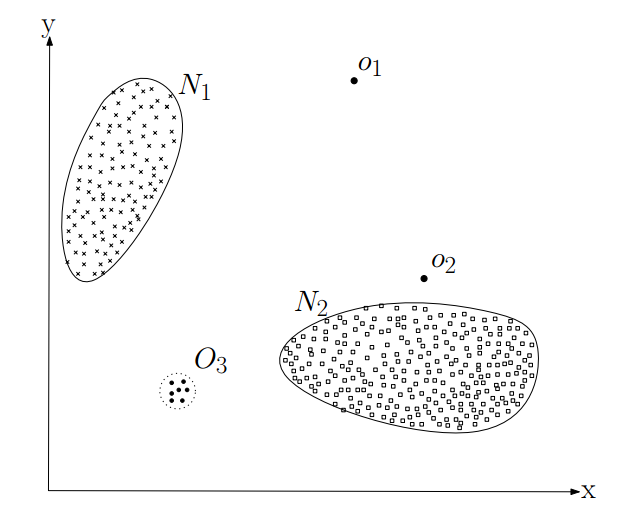
\includegraphics[width=0.5\textwidth]{fig_anomalias.png}
		\end{center}
	\legend{Fonte: \cite{AnomalyDetectionSurvey2009}}
	\label{fig_anomalias}
\end{figure}

\subsection{Tipos de Anomalias}
\label{anom_types}
Determinar o tipo de anomalia sendo identificado é um aspecto importante das técnicas de detecção de anomalias. As anomalias podem ser classificadas em 3 tipos: Pontuais, Contextuais e Coletivas.

Quando uma observação individual é considerada anômala em relação ao restante dos dados, ela é chamada de \textbf{anomalia pontual} \cite{AnomalyDetectionSurvey2009}. Esse tipo de anomalia é o foco da maioria das aplicações e pesquisas na área de detecção de anomalias. Na Figura~\ref{fig_anomalias}, os pontos $o_1$ e $o_2$ são anomalias pontuais. Por exemplo, em um conjunto de dados com valores de umidade relativa coletadas durante uma semana, pode-se ter leituras normais entre 30\% e 50\% e apenas uma leitura com valor 90\%, que é uma anomalia pontual. 

\bigskip
\begin{figure}
	\caption{Exemplo de anomalia contextual.}
	\bigskip
		\begin{center}
			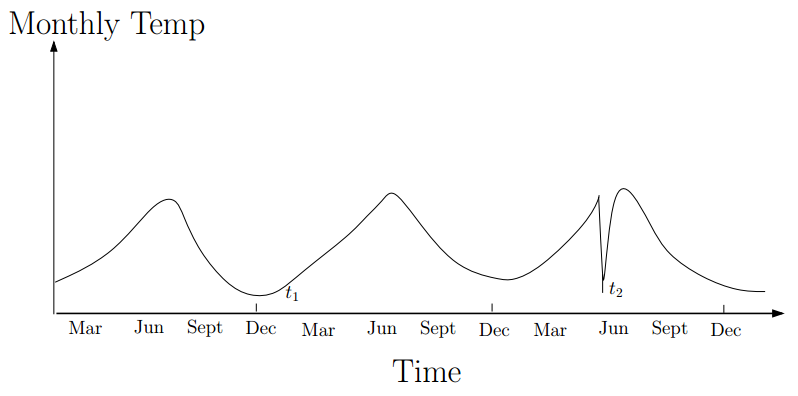
\includegraphics[width=0.7\textwidth]{fig_contextuais.png}
		\end{center}
	\legend{Fonte: \cite{AnomalyDetectionSurvey2009}}
	\label{contextuais}
\end{figure}

Quando uma instância de dado é considerada anômala dentro de um contexto específico, ela é uma \textbf{anomalia contextual} \cite{AnomalyDetectionSurvey2009}. Por exemplo, um sensor de temperatura pode ter leituras altas durante o dia e baixas durante a noite. Embora uma leitura alta não seja necessariamente uma anomalia, se ela ocorreu durante a noite, então é uma anomalia com respeito ao contexto da hora do dia. Nesse caso, cada instância de dado é definida usando conjuntos de \textbf{atributos contextuais}, que indicam o contexto daquela instância (como \textit{Hora do Dia}), e \textbf{atributos comportamentais}, que definem as características independentes de contexto da instância (como \textit{Temperatura}). A Figura~\ref{contextuais} mostra um exemplo de anomalia contextual. A temperatura $t_2$ tem o mesmo valor que $t_1$, porém, devido ao seu contexto, $t_2$ é uma anomalia.

Quando um conjunto de observações é anômalo em relação ao restante do conjunto de dados, ele é chamado de \textbf{anomalia coletiva} \cite{AnomalyDetectionSurvey2009}. As observações individuais dentro desse conjunto podem não ser anomalias por si, mas sua ocorrência em conjunto ou sequência é anômala. Por exemplo, se durante o dia sabe-se que a temperatura sobe de 20$^{\circ}$C pela manhã até 35$^{\circ}$C ao meio dia e desce novamente até 20$^{\circ}$C no fim da tarde, um dia em que a temperatura permaneça em 20$^{\circ}$C durante esse período, contém uma anomalia coletiva. O valor de 20$^{\circ}$C não é anômalo por si, mas sua ocorrência durante todo o período citado faz desse conjunto uma anomalia. A Figura~\ref{coletivas} mostra uma anomalia coletiva em um eletrocardiograma humano \cite{Goldberger}. Os valores da região vermelha não são anômalos individualmente, mas sua ocorrência em sequência caracteriza essa região como uma anomalia.


\begin{figure}
	\caption{Exemplo de anomalia coletiva.}
		\begin{center}
			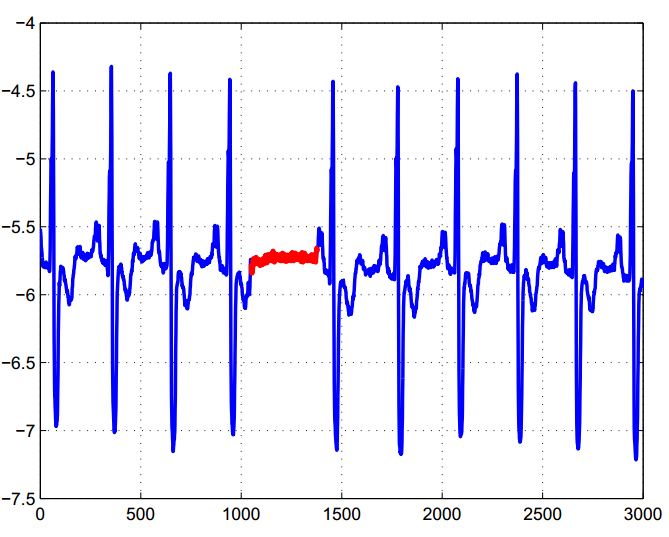
\includegraphics[width=0.6\textwidth]{fig_coletivas.png}
		\end{center}
	\legend{Fonte: \cite{Goldberger}}
	\label{coletivas}
\end{figure}


\subsection{Métricas}
\label{metrics}
No Capítulo 4, algumas métricas são utilizadas para a avaliação da implementação do detector de anomalias. Essas métricas são a matriz de confusão e o \textit{F-score}. A matriz de confusão, ou matriz de erro, é uma tabela que permite a visualização da performance de um algoritmo de classificação através do número de instâncias que foram classificadas corretamente. Cada coluna da tabela representa as instâncias classificadas em determinada classe enquanto cada linha representa a classe real da instância. Portanto, nessa tabela podem ser identificadas as quantidades de verdadeiros positivos, falsos positivos, verdadeiros negativos e falsos negativos classificados pelo detector. "Positivos", no contexto de detecção de anomalia, são os dados anômalos. A Tabela~\ref{confusion_m} mostra a estrutura de uma matriz de confusão para uma classificação binária.

\begin{table}[h]
    \caption{Matriz de Confusão}
    \bigskip
    \begin{center}
        \begin{tabular}{|o|c|c|}
          \hline
          \rowcolor{darkorange}
          \textit{ } & \textit{Classificados como Anomalia} & \textit{Classificados como Normal} \\
          \hline
          \textit{Verdadeiras Anomalias} & Verdadeiros Positivos & Falsos Negativos\\
          \hline
          \textit{Verdadeiros Normais} & Falsos Positivos & Verdadeiros Negativos\\
          \hline
        \end{tabular}
    \label{confusion_m}
    \end{center}
\end{table}

O \textit{F-score} é utilizado para medir a precisão de um teste de classificação binária. Basicamente, o \textit{F-score} é a média harmônica entre a Precisão e a Revocação (também conhecida como Sensibilidade) \cite{modern1999}. A Precisão é a fração dos elementos recuperados que são relevantes. A Revocação é a fração dos elementos recuperados do total de elementos relevantes. As Equações~\ref{precision}, \ref{recall} e \ref{fscore} mostram o cálculo da Precisão, Revocação e do \textit{F-score}, respectivamente.

\begin{equation}
    \label{precision}
    \textrm{Precisão} = \frac{\textrm{Verdadeiros Positivos}}{\textrm{Verdadeiros Positivos} + \textrm{Falsos Positivos}}
\end{equation}

\begin{equation}
    \label{recall}
    \textrm{Revocação} = \frac{\textrm{Verdadeiros Positivos}}{\textrm{Verdadeiros Positivos} + \textrm{Falsos Negativos}}
\end{equation}

\begin{equation}
    \label{fscore}
    \textrm{\textit{F-score}} = 2\cdot\frac{\textrm{Precisão} \cdot \textrm{Revocação}}{\textrm{Precisão} + \textrm{Revocação}}
\end{equation}

\section{Técnicas de Detecção de Anomalias}
\label{anom_tec}
Nesta Seção, diversas técnicas de detecção de anomalias normalmente utilizadas no contexto de redes de sensores são apresentadas. Anomalias identificadas em dados de sensores podem indicar que um ou mais sensores estão defeituosos ou que eventos que podem ser interessantes para analistas estão ocorrendo, como intrusões \cite{AnomalyDetectionSurvey2009}. Existem alguns desafios para a detecção de anomalias em redes de sensores. A presença de ruído devido as condições hostis em que sensores operam e o fato de os dados serem coletados de fontes distribuídas tornam a detecção de anomalias mais difícil.

\subsection{Anotação de Dados}
Instâncias de dados podem ter anotações associadas que indicam se a observação é normal ou anômala. Geralmente esse tipo de anotação é feita por um especialista humano, portanto é muito difícil e cara de ser obtida. É mais difícil obter um conjunto de dados com anotações para todos os tipos de anomalias do que obter anotações de dados normais. Dependendo da disponibilidade e do tipo de anotações disponíveis, os algoritmos de detecção de anomalias operam em três categorias \cite{AnomalyDetectionSurvey2009}:

\begin{itemize}
    
    \item \textit{Detecção de Anomalias Supervisionada} - Técnicas de treinamento supervisionado necessitam de um conjunto de dados com anotações para as instâncias normais e anômalas. Desse modo, o problema se torna similar ao aprendizado de um modelo preditivo. Cada nova instância é comparada com o modelo para a determinação de sua classe (normal ou anomalia). Dois problemas surgem ao se utilizar métodos de treinamento supervisionado no contexto de detecção de anomalias. Na maioria das aplicações, é muito difícil obter anotações precisas e representativas, especialmente para a classe anômala. Além disso, o número de anomalias presentes em um conjunto de dados é muito menor do que as instâncias normais, o que pode prejudicar o treinamento e validação de modelos preditivos.

    \item \textit{Detecção de Anomalias Semi-supervisionada} - Técnicas semi-supervisionadas são mais abrangentes do que técnicas supervisionadas porque elas só dependem de anotações para os dados normais do conjunto. Normalmente elas consistem na construção de um modelo preditivo para a classe normal dos dados e no uso desse modelo para a identificação de anomalias.

    \item \textit{Detecção de Anomalias Não Supervisionada} - Técnicas não supervisionadas não dependem de um conjunto de dados anotado, portanto são as mais abrangentes. Essas técnicas assumem que instâncias de dados normais aparecem com muito mais frequência no conjunto do que dados anômalos. Se essa suposição não for correta, essas técnicas sofrem de um grande número de falsos negativos.

\end{itemize}


\subsection{Técnicas de Detecção de Anomalias}
Esta Seção descreve as principais técnicas de detecção de anomalias utilizadas em redes de sensores, definidas baseadas em \cite{AnomalyDetectionSurvey2009}.

\subsubsection{Redes Bayesianas}
Técnicas de detecção de anomalias baseadas em Redes Bayesianas (RB) normalmente são utilizadas em cenários com múltiplas classes. A técnica básica utiliza uma RB "ingênua" para estimar a probabilidade de uma nova instância de dado ser classificada em cada classe a partir de um conjunto de treinamento com anotações das classes normais e das classes anômalas. A classe com a maior probabilidade é então selecionada para a dada observação.

A técnica básica, univariada, pode ser estendida para conjuntos de dados multivariados agregando-se as probabilidades estimadas de cada atributo do novo dado e utilizando-se esse novo valor para atribuir uma classe ao novo dado. Essa técnica assume independência entre os diferentes atributos. \cite{BayesianBelief} utiliza RBs mais complexas para capturar as dependências entre atributos.

\subsubsection{Sistemas Baseados em Regras}
Técnicas de detecção de anomalias baseadas em regras focam em aprender regras que descrevem o comportamento normal de um sistema. Uma instância de teste que não é capturada por nenhuma regra é considerada uma anomalia \cite{ContextualMichael2014}.

Para cenários com múltiplas classes, o método básico consiste em extrair as regras utilizando um algoritmo de aprendizado de regras (Árvores de Decisão, RIPPER \cite{cohen1995fast}). A cada regra é associado um valor de confiança, dependendo do número de instâncias que foram corretamente classificadas pela regra durante o treinamento. Ao se testar um novo valor, encontra-se a melhor regra que o captura. O inverso do valor de confiança dessa regra é a pontuação de anomalia do novo dado.

\subsubsection{Modelagem Estatística Paramétrica}
Qualquer técnica estatística de detecção de anomalias se baseia no princípio de que dados normais ocorrem nas áreas de maior probabilidade de um modelo estocástico enquanto anomalias ocorrem nas áreas de baixa probabilidade \cite{AnomalyDetectionSurvey2009}. Essas técnicas encaixam um modelo estatístico no conjunto de treinamento (normalmente as instâncias normais) e então aplicam uma inferência estatística para determinar se a instância de teste pertence à área de alta probabilidade do modelo.

Existem dois tipos de modelagens: não-paramétricas e paramétricas. Modelagens não-paramétricas fazem poucas suposições sobre a distribuição dos dados e incluem técnicas baseadas em histogramas e \textit{kernel}. Modelagens paramétricas assumem que os dados normais são gerados por uma distribuição paramétrica. Exemplos incluem o modelo Gaussiano e o modelo de regressão \cite{AnomalyDetectionSurvey2009}. Os parâmetros da distribuição são estimados a partir do conjunto de treinamento. O inverso do valor da função de distribuição aplicada a uma nova instância é a pontuação de anomalia daquela instância.

\subsubsection{Técnicas baseadas na Vizinhança Próxima}
Técnicas baseadas na vizinhança próxima assumem que as instâncias de dados normais ocorrem em áreas de maior densidade, enquanto anomalias ocorrem longe de seus vizinhos mais próximos \cite{AnomalyDetectionSurvey2009}. A definição da métrica de similaridade (distância) utilizada na comparação de duas instâncias de dado é um dos fatores mais importantes para o desempenho desse tipo de técnica. Para atributos contínuos, pode-se utilizar distância Euclidiana, distância de Manhattan ou outra. Para atributos categóricos, outras métricas podem ser usadas, como a distância de Hamming. No caso de dados multivariados, a distância é calculada para cada atributo individualmente e então é combinada. A distância de uma instância de dado para o seu k-ésimo vizinho mais próximo pode ser utilizada como sua pontuação de anomalia.

\section{Trabalhos Relacionados}
\label{trab_rel}
Vários trabalhos científicos abordam o problema da detecção de anomalias em redes de sensores. Devido à natureza dessas redes, normalmente esses trabalhos propõem algoritmos distribuídos, que são executados em cada nodo da rede, e há uma preocupação com a escalabilidade. Esta seção descreve trabalhos relacionados à detecção de anomalias em redes de sensores

\subsection{Descrição dos Trabalhos Relacionados}
O método proposto por \cite{Ellipsoids2009} realiza detecção de anomalias em uma rede de sensores através do agrupamento de elipsoides. Primeiramente, cada nodo (sensor) da rede estima um elipsoide local para sua distribuição de valores e envia os parâmetros para a base. Na base, é realizado um agrupamento dos elipsoides locais, de forma a eliminar elipsoides redundantes. Para cada grupo, a base cria um elipsoide que envolva todos os elipsoides do grupo. Esses elipsoides globais são enviados para os nodos da rede, que os utilizam para marcar anomalias globais. Alguns desafios do método são a escolha do número de grupos e a escolha da métrica de similaridade entre os elipsoides.

\cite{DistributedFuzzy2013} propõe um algoritmo distribuído de detecção de anomalias que utiliza agrupamento nebuloso. Primeiramente, é modelada uma arquitetura hierárquica a partir dos nodos da rede, resultando em uma árvore com diferentes níveis de granularidade.~Cada nodo utiliza o algoritmo \textit{fuzzy c-means} para agrupar suas observações locais coletadas durante um período de tempo $\Delta t$ . O grau de pertinência para cada grupo é calculado e as anomalias locais são identificadas utilizando-se um limite estatístico.~Cada nodo envia as anomalias identificadas e os grupos para seus nodos pais, que combinam a informação recebida com seus próprios resultados de agrupamento e identificação de anomalias. Esse processo é repetido até que se chegue ao nodo raiz, que possuirá as informações de todas as anomalias globais e locais. Através de seus filhos, o nodo raiz envia as anomalias globais de volta para os nodos individuais, que usam a informação para realizar a identificação de anomalias localmente. O algoritmo se mostrou preciso. Uma desvantagem é que a definição do número de grupos deve ser feita no nível local.

\cite{BayesianBelief} utiliza Redes Bayesianas (RB) para a detecção de anomalias em redes de sensores. Primeiramente, uma RB é construída modelando-se a dependência entre os atributos dos sensores (por exemplo, o atributo \textit{Umidade} pode depender do atributo \textit{Temperatura}). Essa dependência pode ser obtida através do conhecimento humano ou através da busca entre possíveis estruturas. Em seguida, o intervalo de normalidade de cada atributo é dividido em classes e a distribuição de probabilidade para cada atributo é estimada. Essa informação compõe uma tabela de probabilidade condicional que é mantida em cada nodo da rede. Cada novo valor $X$ é testado calculando-se a probabilidade de $X$ pertencer a alguma classe. A classe com a maior probabilidade é selecionada e comparada com $X$. Se $X$ estiver fora do intervalo da classe, $X$ é marcado como anomalia.

\cite{hbos2012} propõe um método de detecção de anomalias não supervisionado baseado em histogramas.~Primeiramente, um histograma é construído para cada dimensão do banco de dados. Os histogramas podem ser discretos (para dados categóricos, por exemplo) ou contínuos. Se o atributo for contínuo, o histograma pode ter barras de largura fixa ou a largura pode ser determinada dinamicamente. Após a construção dos histogramas, a pontuação de anomalia de cada instância é calculada de acordo com a altura das barras dos histogramas que englobam seus valores de atributos. Essa pontuação é comparada com um valor limite escolhido durante a implementação para a determinação da normalidade da instância. A maior vantagem do método é que ele é extremamente rápido em relação a outros métodos não supervisionados, porém não é capaz de detectar anomalias locais.

\cite{ContextualMichael2014} apresenta um \textit{framework} para a detecção contextual de anomalias dividido em duas partes: um componente de detecção pontual e outro de detecção contextual de anomalia. Esse \textit{framework} é reproduzido e avaliado no presente trabalho. O Capítulo~\ref{cap_baseline} descreve esse trabalho em detalhes.

\subsection{Comparativo entre os Trabalhos Relacionados}
A Tabela~\ref{comparativo} estabelece comparações entre atributos dos trabalhos relacionados apresentados. Enquanto a maioria dos trabalhos oferece uma solução distribuída, o trabalho de \citeauthor{ContextualMichael2014} é o único que considera o contexto dos dados. As técnicas utilizadas por cada trabalho são variadas. A maioria dos algoritmos de detecção de anomalias é de aprendizado não supervisionado. É difícil classificar todos os tipos de anomalias que podem ocorrer, portanto é comum buscar agrupar os dados normais e utilizar esse agrupamento ou modelagem para a detecção de anomalias.

\begin{table}[h]
\begin{adjustwidth}{-0.8in}{-1in}
    \caption{Comparação entre os Trabalhos Relacionados}
    \bigskip
    \begin{center}
        \begin{tabular}{|o|c|c|P{2.5cm}|c|}
          \hline
          \rowcolor{darkorange}
          Trabalho & Considera Contexto & Processamento & Técnica & Aprendizado\\
          \hline
          \citeauthor{Ellipsoids2009} & Não & Distribuído & Modelagem Paramétrica & Não Supervisionado\\
          \citeauthor{DistributedFuzzy2013} & Não & Distribuído & Vizinhança Próxima & Não Supervisionado\\
          \citeauthor{BayesianBelief} & Não & Distribuído & Redes Bayesianas & Supervisionado\\
          \citeauthor{hbos2012} & Não & Centralizado & Modelagem Não-Paramétrica & Não Supervisionado\\
          \citeauthor{ContextualMichael2014} & Sim & Centralizado & Modelagem Paramétrica & Não Supervisionado\\
          \hline
        \end{tabular}
    \label{comparativo}
    \end{center}
\end{adjustwidth}
\end{table}

% ========== CAP 3 ==============
\chapter{Descrição do \textit{Baseline}}
\label{cap_baseline}
Este capítulo detalha o trabalho desenvolvido por \citeauthor{ContextualMichael2014} descrito em \cite{ContextualMichael2014}, um Framework para a Detecção Contextual de Anomalias (FDCA). O trabalho descreve um \textit{framework} para a detecção de anomalias em dados de sensores levando em conta o contexto dos dados. O trabalho foi selecionado como base pois oferece uma solução flexível, modularizada e busca atender as limitações e requerimentos próprios do contexto de \textit{Big Data}, em que centenas de milhares de dados precisam ser avaliados a cada segundo. A técnica possui dois componentes: um detector de anomalias pontuais e um detector de anomalias contextuais. Ambos componentes são descritos a seguir.


\begin{figure}
	\caption{\textit{Framework} para a Detecção de Anomalias Contextuais - FDCA}
	\bigskip
		\begin{center}
			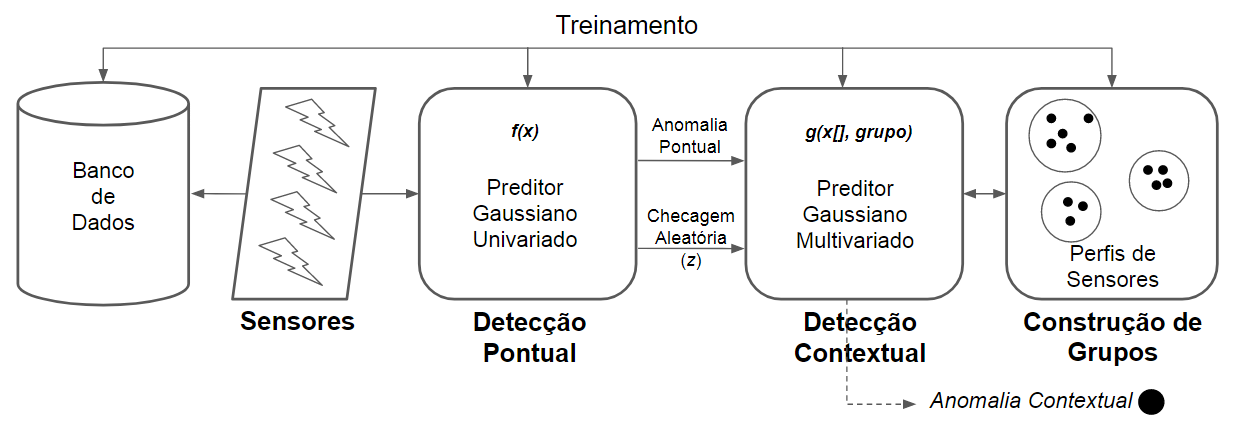
\includegraphics[width=1\textwidth]{CADF.PNG}
		\end{center}
	\legend{Fonte: \cite{ContextualMichael2014}}
	\label{cadf_arq}
\end{figure}


\section{Visão Geral}
O \textit{framework} proposto por \cite{ContextualMichael2014} divide o processo de detecção de anomalias em dois passos: primeiro, os dados de entrada são avaliados pelo detector pontual de anomalias, que é rápido, porém impreciso. O objetivo dessa primeira etapa é capturar todas as verdadeiras anomalias, mesmo que algumas falsas anomalias sejam capturadas também. Depois, os dados marcados como anomalias pelo detector pontual são avaliados pelo detector contextual, que é mais lento, porém mais preciso que o pontual. Os dados que continuarem anotados como anômalos após o segundo passo são os reportados como anômalos pelo \textit{framework}. Também existe um fator aleatório que permite que dados marcados como normais pelo detector pontual sejam enviados para o detector contextual. O objetivo é encontrar valores que estejam agindo normalmente em sua vizinhança, mas não quando vistos em relação ao seu contexto. 

O principal motivo para essa divisão é a busca da escalabilidade do \textit{framework} para grandes volumes de dados. Embora a avaliação contextual possa ser lenta, apenas as instâncias marcadas como anômalas pelo avaliador pontual são analisados contextualmente. Isso significa que o \textit{framework} consegue avaliar observações com uma velocidade satisfatória mesmo para grandes volumes e velocidade de dados. A Figura~\ref{cadf_arq} mostra a arquitetura do FDCA. O banco de dados salva as leituras dos sensores, que são utilizadas no treinamento. O componente de detecção pontual avalia os novos valores de sensores e envia os que forem classificados como anomalias para o componente de detecção contextual. O componente de construção de grupos constrói os perfis de sensores e fornece essa informação para o componente de detecção contextual.

Os Algoritmos~\ref{alg_1}, \ref{alg_2} e \ref{alg_3} mostram o funcionamento geral do \textit{framework}. O algoritmo recebe como entrada a leitura do valor do sensor e sua informação contextual e devolve uma anotação que determina se essa leitura é normal ou anômala. O algoritmo também recebe a probabilidade de checar se a leitura é contextualmente anômala mesmo que ela seja considerada pontualmente normal. O primeiro passo é realizar a detecção pontual, comparando o valor do PreditorGaussianoUnivariado com o $\epsilon$ do componente de detecção pontual, como mostra o Algoritmo~\ref{alg_2}. Se esse resultado for positivo ou for acionada a detecção contextual aleatória (Algoritmo~\ref{alg_1}, linha 5), o perfil do sensor é recuperado e se realiza a detecção contextual. Na detecção contextual, representada no Algoritmo~\ref{alg_3}, o PreditorGaussianoMultivariado do perfil correspondente à leitura é recuperado e então seu valor é comparado com o $\epsilon$ do componente da detecção contextual. Finalmente, se o resultado dessa comparação for positivo, a leitura do sensor é anotada como anômala.

A Seção~\ref{anom_pont} detalha o processo de detecção pontual e a Seção~\ref{anom_contxt} detalha o processo de detecção contextual e a criação de Perfis de Sensores, processo que busca simplificar a detecção contextual de anomalias. 

\bigskip
\begin{algorithm}
\caption{FDCA}
\label{alg_1}
\begin{algorithmic}[1]
\Procedure{Detec\c{c}\~aoContextualDeAnomalia}{}
\State $\textit{valorSensor} \gets \text{Leitura do sensor}$
\State $\textit{contextoSensor} \gets \text{Contexto da leitura do sensor}$
\State $z \gets \text{Probabilidade de checar diretamente se é anomalia contextual}$
\If {$\text{\'EAnomaliaPontual}(valorSensor) \text{ \textbf{or} } z \leq \text{Random()}$}
\State $\text{\textit{perfilSensor}} \gets \text{PerfilDoSensor(\textit{valorSensor}, \textit{contextoSensor})}$
\If {$\text{\'EAnomaliaContextual(\textit{valorSensor}, \textit{contextoSensor}, \textit{perfilSensor})}$}
\State \Return $\text{Dado An\^omalo}$
\Else
\State \Return $\text{Dado Normal}$
\EndIf
\Else
\State \Return $\text{Dado Normal}$
\EndIf
\EndProcedure
\end{algorithmic}
\end{algorithm}

\begin{algorithm}
\caption{Detecção Pontual de Anomalia}
\label{alg_2}
\begin{algorithmic}[1]
\Procedure{\'EAnomaliaPontual}{valorSensor}
\If {$\text{PreditorGaussianoUnivariado}(valorSensor) < \epsilon$}
\State \Return $\text{True}$
\Else
\State \Return $\text{False}$
\EndIf
\EndProcedure
\end{algorithmic}
\end{algorithm}

\begin{algorithm}
\caption{Detecção Contextual de Anomalia}
\label{alg_3}
\begin{algorithmic}[1]
\Procedure{\'EAnomaliaContextual}{valorSensor, contextoSensor, perfilSensor}
\State $\text{PreditorGaussianoMultivariado} \gets \text{PreditorDoPerfil(\textit{perfilSensor})}$
\If {$\text{PreditorGaussianoMultivariado}(\textit{valorSensor}, \textit{contextoSensor}) < \epsilon$}
\State \Return $\text{True}$
\Else
\State \Return $\text{False}$
\EndIf
\EndProcedure
\end{algorithmic}
\end{algorithm}

\section{Detecção de Anomalia Pontual}
\label{anom_pont}
O \textit{framework} utiliza modelagem paramétrica para a detecção de anomalias pontuais. Em particular, uma distribuição Gaussiana de probabilidade é calculada a partir do histórico dos dados. Esse componente do \textit{framework} também é chamado de Preditor Gaussiano Univariado. "Univariado"~porque apenas os valores comportamentais dos sensores são levados em consideração para a estimação da distribuição, ignorando-se o contexto. Isso assegura que o preditor pode classificar novos valores rapidamente, sacrificando precisão \cite{ContextualMichael2014}. O componente de detecção contextual de anomalias lida com o problema da precisão.

O Preditor Gaussiano Univariado utiliza dois parâmetros extraídos do conjunto de dados: a média, $\mu$, e a variância, $\sigma^2$, de cada atributo. As Equações~\ref{uni_mean} e \ref{uni_var} mostram como esses parâmetros são calculados, onde $m$ é o número de observações de treinamento e $x^{(i)}$ é o valor do sensor para a observação de treinamento $i$. A Equação~\ref{uni_pdf} é utilizada para a avaliação de novos valores, onde $n$ é o número de atributos comportamentais do dado $x$. Um dado $x$ é considerado anômalo se $p(x) < \epsilon$, onde $\epsilon$ é um valor escolhido durante a implementação.

\begin{equation}
    \label{uni_mean}
    \mu = \frac{1}{m} \sum_{i=1}^{m} x^{(i)}
\end{equation}

\begin{equation}
    \label{uni_var}
    \sigma^2 = \frac{1}{m} \sum_{i=1}^{m} (x^{(i)} - \mu)^2
\end{equation}

\begin{equation}
    \label{uni_pdf}
    p(x) = \prod_{j=1}^{n} \frac{1}{\sqrt{2\pi\sigma^2}}\exp{-\frac{(x_j - \mu_j)}{2\sigma^2}}
\end{equation}

\section{Detecção de Anomalia Contextual}
\label{anom_contxt}
A detecção de anomalia contextual é baseada em dois processos: a definição de perfis de sensores e a atribuição de cada valor de sensor a um perfil; e a comparação de uma nova leitura de sensor (já declarada anômala pelo detector pontual) com a média esperada pelo perfil correspondente ao sensor \cite{ContextualMichael2014}. A Seção~\ref{sensor_prof} detalha a construção dos perfis de sensores, enquanto a Seção~\ref{pred_multi} explica o Preditor Gaussiano Multivariado, componente utilizado na detecção contextual de anomalias.

\subsection{Perfis de Sensores}
\label{sensor_prof}
A criação dos perfis de sensores é realizada utilizando-se um algoritmo multivariado de agrupamento que divide as leituras presentes no histórico em grupos que se comportam de maneira similar. O algoritmo é multivariado para incluir informações contextuais sobre as leituras, como dia da semana, hora do dia, posição, andar, mês. Para lidar com o grande volume de dados presente no contexto de \textit{Big Data}, o algoritmo de agrupamento é executado de acordo com um modelo de paralelismo conhecido como \textit{MapReduce} \cite{mapreduce2008}, que consiste de dois procedimentos: \textit{Map()} e \textit{Reduce()}. No primeiro, os dados são divididos em partes menores e processados separadamente. No segundo, os resultados dos procedimentos \textit{Map()} são agregados.

Na construção dos perfis de sensores, são realizadas duas iterações de \textit{MapReduce}. No primeiro procedimento \textit{Map()}, os dados são divididos em $n$ partes e cada parte é utilizada como entrada para o algoritmo \textit{k-means}, gerando $n \cdot k$ grupos. Os centroides desses grupos são utilizados no primeiro procedimento \textit{Reduce()} como entrada para outra chamada do algoritmo \textit{k-means}, gerando $k$ grupos finais correspondentes aos perfis de sensores. O segundo procedimento \textit{Map()} apenas atribui cada perfil a um grupo de dados. Finalmente, o segundo procedimento \textit{Reduce()} cria um Preditor Gaussiano Multivariado para cada subconjunto de leituras pertencente a cada perfil de sensor.

O algoritmo \textit{k-means} busca dividir um conjunto de pontos de dados em $k$ grupos de forma a minimizar a soma dos quadrados das distâncias dentro de cada grupo. O algoritmo \textit{k-means} segue os seguintes passos:

\begin{enumerate}
    \item Inicie $k$ centroides aleatoriamente.
    \item Divida o conjunto de dados em $k$ grupos, colocando cada instância no grupo cujo centroide é mais próximo, de acordo com a Equação~\ref{k_means}.
    \item Recalcule o valor do centroide de cada grupo.
    \item Repita os passos 2 a 3 até que os valores dos centroides não sejam modificados.
\end{enumerate}

\begin{equation}
    \label{k_means}
    \min_s \sum_{i=1}^k \sum_{x_j} ||x_j - \mu_i||^2
\end{equation}

\subsection{Preditor Gaussiano Multivariado}
\label{pred_multi}
Da mesma forma que a detecção pontual, a detecção contextual de anomalias cria um modelo paramétrico dos dados e o utiliza para separar as amostras. Uma distribuição Gaussiana multivariada é estimada a partir da média e variância do histórico dos dados. As Equações~\ref{multi_mean} e \ref{multi_var} mostram como os parâmetros da distribuição são obtidos. A Equação~\ref{multi_pdf} é utilizada para a avaliação de novas instâncias de dados. A nova instância $x$ é considerada anômala se $p(x) < \epsilon$ onde $\epsilon$ é um valor escolhido durante a implementação. $\Sigma$, na Equação~\ref{multi_pdf}, é a matriz de covariância dos atributos utilizados para a estimativa da distribuição Gaussiana multivariada e $|\Sigma|$ é o determinante dessa matriz. $m$ é o número de instâncias de treinamento e $n$ é o número de atributos inclusos no cálculo da distribuição Gaussiana multivariada. A distribuição Gaussiana multivariada automaticamente captura correlações entre os atributos do conjunto de dados, justificando o uso de atributos contextuais no cálculo.

\begin{equation}
    \label{multi_mean}
    \mu_j = \frac{1}{m} \sum_{i=1}^{m} x_j^{(i)}
\end{equation}

\begin{equation}
    \label{multi_var}
    \Sigma = \frac{1}{m} \sum_{i=1}^{m} (x_j^{(i)} - \mu_j)(x_j^{(i)} - \mu_j)^T
\end{equation}

\begin{equation}
    \label{multi_pdf}
    p(x) = \frac{1}{\sqrt{2\pi^{n}|\Sigma|}}\exp{(-\frac{1}{2}(x - \mu)^T\Sigma^{-1}(x - \mu))}
\end{equation}

\section{Fator Aleatório}
\label{fator_aleatorio}
O componente de detecção pontual pode, aleatoriamente, marcar uma instância como anômala mesmo que a Detecção de Anomalia Pontual declare ela como normal. O objetivo é encontrar instâncias que são anomalias apenas quando observadas em relação ao seu contexto, diminuindo o número de falsos negativos. A probabilidade $z$ de uma instância ser enviada diretamente para o detector contextual é definida durante a implementação.

\section{Discussões}
Algumas das vantagens do \textit{framework} apresentado neste Capítulo são a modularidade, o que o torna bastante flexível, e a escalabilidade. A modularidade permite que alterações sejam feitas em vários momentos, adequando o \textit{framework} para um problema específico. A escalabilidade, obtida através da combinação da detecção pontual e detecção contextual, permite que o \textit{framework} opere bem mesmo quando a rede é formada por um conjunto grande de sensores. Um dos pontos a serem trabalhados no \textit{framework} é o fator aleatório. Se um valor estático pequeno for utilizado, como $0,001$, a probabilidade de uma anomalia verdadeira ser enviada para a detecção contextual é quase insignificante, dado que anomalias, por definição, são eventos muito raros. Outro ponto fraco do sistema é que os componentes assumem distribuição normal dos dados, o que raramente ocorre no mundo real.

% ========== CAP 4 ==============
\chapter{Implementação do Detector Contextual de Anomalias}
\label{implementacao}
Este capítulo descreve a implementação do FDCA. O \textit{framework} foi implementado utilizando a linguagem de programação \textit{Python}, com uso das bibliotecas \textit{Scikit-learn} \cite{scikit-learn}, \textit{Pandas} \cite{mckinney-proc-scipy-2010}, \textit{Numpy} \cite{walt2011numpy} e \textit{Matplotlib} \cite{hunter2007matplotlib}. A arquitetura é formada por um componente de construção de perfis de sensores e um componente de detecção de anomalia. O componente de detecção de anomalia possui um componente de detecção de anomalia pontual e um componente de detecção de anomalia contextual, como descrito no Capítulo~\ref{cap_baseline}. A Seção~\ref{imp_vis_geral} detalha cada componente da arquitetura. As Seções~\ref{mod_1} e \ref{mod_2} apresentam as modificações sugeridas.

\section{Visão Geral}
\label{imp_vis_geral}
A Figura~\ref{imp_arq} ilustra a arquitetura da implementação. O componente de detecção de anomalia possui dois subcomponentes, um componente de detecção pontual e um componente de detecção contextual, de modo que é possível realizar a avaliação com apenas um dos componentes ou com a combinação dos dois, formando o FDCA efetivamente. A construção de perfis de sensores é um componente à parte e, após realizar o agrupamento, fornece a informação de quais dados de treinamento pertencem a cada perfil e um classificador que permite recuperar o perfil de novos dados de entrada. O treinamento e avaliação divide o conjunto de entrada em treinamento e teste e realiza a avaliação através de validação cruzada.

\begin{figure}
	\caption{Arquitetura do FDCA}
	\bigskip
		\begin{center}
			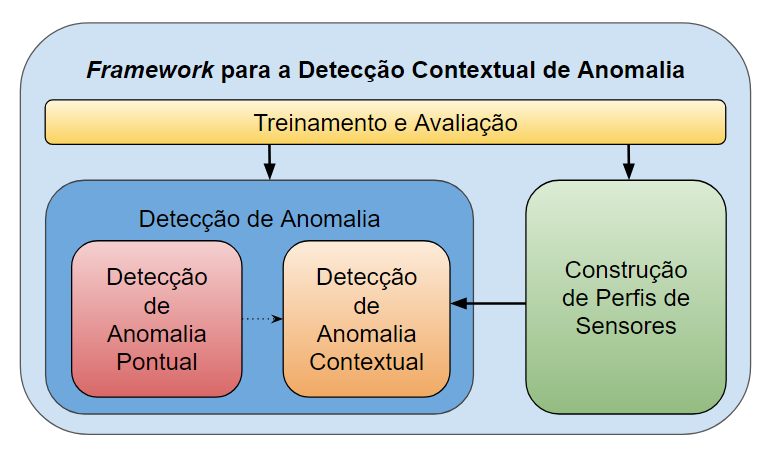
\includegraphics[width=0.68\textwidth]{arq.png}
		\end{center}
	\label{imp_arq}
\end{figure}

\subsection{Construção de Perfis de Sensores}
\label{construcao_sp}
O componente de construção de perfis de sensores é responsável pelo agrupamento dos dados de treinamento em $k$ grupos e pela criação de um Preditor Gaussiano Multivariado para cada grupo. Esse processo é feito seguindo o modelo \textit{MapReduce}, conforme descrito na Seção~\ref{sensor_prof}. Para cada chamada do procedimento \textit{Map()}, uma \textit{thread} é criada, de forma a acelerar o agrupamento. Para o agrupamento, é utilizada a classe \textit{KMeans} da biblioteca \textit{Scikit-learn} e o algoritmo é executado sobre o conjunto de treinamento normalizado.

Após o agrupamento, os dados são remapeados para seus respectivos grupos e então é criado um Preditor Gaussiano Multivariado para cada grupo. Com a informação dos dados pertencentes a cada grupo, os parâmetros de cada distribuição são estimados, completando o processo de construção dos perfis de sensores.

\subsection{Detecção de Anomalia Pontual}
\label{sistema_pont}
O componente de detecção pontual é responsável por avaliar cada instância de dado utilizando seus atributos comportamentais, isto é, as leituras dos sensores. Durante a fase de treinamento, a média e a variância do conjunto de treinamento são estimadas de acordo com as Equações~\ref{uni_mean} e \ref{uni_var}. Em seguida, o $\epsilon$ é calculado. Porque a Detecção de Anomalia Pontual deve tentar capturar todos os verdadeiros positivos, o $\epsilon$ é escolhido como uma porcentagem do valor máximo da função de densidade de probabilidade, isto é, $p(\mu)$ (Equação~\ref{uni_pdf}).~A função tem valor máximo em $p(\mu)$, portanto $\epsilon = c \cdot p(\mu)$,~onde~$0 \leq c \leq 1$. $c$ pode ser ajustado no intervalo $[0,1]$ para tornar a Detecção Pontual de Anomalia mais ou menos tolerante.

É também no componente de detecção pontual que é decidido se uma instância de dado deve ser avaliada contextualmente independente de ela ser considerada anômala ou não pelo Preditor Gaussiano Univariado. Essa decisão é feita aleatoriamente com base em um parâmetro $z$, como é demonstrado pelo Algoritmo~\ref{alg_1}.

\subsection{Detecção de Anomalia Contextual}
\label{sistema_contxt}
O componente de detecção contextual é responsável por descartar os falsos positivos que passaram pela detecção pontual e manter os verdadeiros positivos. Durante a fase de treinamento, a informação dos dados pertencentes a cada perfil de sensor é recuperada do componente de construção de perfis de sensores. A média e a variância é calculada para cada perfil a partir de seus dados correspondentes de acordo com as Equações~\ref{multi_mean} e \ref{multi_var}. Em seguida, o $\epsilon$ para cada perfil de sensor é escolhido da seguinte forma:

\begin{enumerate}
     \item Primeiro, é calculado o valor de $p(x^{(i)})$ para cada $x^{(i)}$ pertencente ao perfil de sensor.
     \item Os valores de $p(x^{(i)})$ são colocados em ordem crescente.
     \item É escolhido $\epsilon = p(x^{(i=0)})$ (Equação~\ref{multi_pdf}) e calcula-se o \textit{F-score} para a classificação do conjunto de treinamento de acordo com esse $\epsilon$. Isto é, $x^{(i)}$ é considerado anômalo se $p(x^{(i)}) < \epsilon$.
     \item \label{passo} Escolhe-se $\epsilon' = p(x^{(i+1)})$ e é verificado se $\epsilon'$ melhora o \textit{F-score}. Caso positivo, $\epsilon = \epsilon'$.
     \item O passo~\ref{passo} é repetido até que o novo \textit{F-score} seja pior que o anterior.
     
\end{enumerate}

Caso não haja anomalias no conjunto de treinamento para algum perfil de sensor, um valor muito pequeno, normalmente $10^{-12}\cdot p(\mu)$, é atribuído a $\epsilon$. 

\subsection{Treinamento e Avaliação}
O treinamento e a avaliação são realizados através de um processo de validação cruzada estratificada com 10 iterações. Nesse processo, o conjunto de dados é dividido em 10 segmentos, preservando-se em cada segmento a mesma proporção de dados normais e anomalias do conjunto inteiro. Um segmento é separado para o teste e os outros 9 segmentos são utilizados no treinamento. No teste são calculadas a matriz de confusão, a precisão, a revocação e o \textit{F-score}.

\section{Primeira Modificação}
\label{mod_1}
A primeira mudança sugerida diz respeito ao fator aleatório que permite que uma instância de dado seja avaliada pelo componente de detecção contextual mesmo que ela seja considerada normal pelo componente de detecção pontual, definido pelo parâmetro $z$. Com o objetivo de tornar esse fator aleatório mais eficaz, foi criado um modo de definir $z$ dinamicamente, de modo que a probabilidade da avaliação direta seja maior conforme o valor de $p(x)$ (Equação~\ref{uni_pdf}) se afasta do valor de $p(\mu)$:

\begin{equation}
    \label{dinamic_z}
    z_{\textrm{dinâmico}}(x) = \frac{1}{(1 + p(x))^{c}}
\end{equation}

Onde $c$ é uma constante calculada durante o treinamento e seu valor é

\begin{equation}
    \label{const_c}
    c = \log_{1 + p(\mu)} 10^{-15}
\end{equation}

A Equação~\ref{dinamic_z} atribui a $z$ um valor entre 0 e 1 que é mais próximo de 1 conforme o valor de $p(x)$ se aproxima de 0, e é mais próximo de 0 conforme o valor de $p(x)$ se aproxima de $p(\mu)$. A constante $c$ calculada através da Equação~\ref{const_c} ajusta a Equação~\ref{dinamic_z} de forma que o valor de $z$ seja $10^{-15}$ quando $p(x)$ é igual a $p(\mu)$.

\section{Segunda Modificação}
\label{mod_2}
A segunda mudança sugerida diz respeito à suposição inicial do \textit{framework} de que os dados seguem uma distribuição normal. O componente de detecção contextual modela os dados de acordo com distribuições gaussianas multivariadas, portanto experimentou-se realizar o processo de agrupamento durante a criação de perfis de sensores modelando os dados como uma mistura Gaussiana. Um modelo de mistura Gaussiana é um modelo probabilístico que assume que os dados foram gerados a partir de uma mistura de distribuições Gaussianas com parâmetros desconhecidos.\footnote{\url{http://scikit-learn.org/stable/modules/mixture.html} Acesso em Julho de 2017}~A classe \textit{BayesianGaussianMixture} da biblioteca \textit{Scikit-learn} é utilizada para a estimação dos modelos.

\section{Limitações}
A limitação da primeira mudança é o seu tempo de execução. O cálculo de $z_{\textrm{dinâmico}}$ é muito lento, portanto fere uma das vantagens do algoritmo, que é a escalabilidade. A segunda mudança pode piorar o desempenho do \textit{framework} se os dados se afastarem o bastante de uma distribuição normal.

\section{Considerações Finais}
Este Capítulo apresentou os detalhes da implementação do FDCA realizada durante o desenvolvimento deste trabalho. Também foram apresentados detalhes de implementação, como a seleção do $\epsilon$ nos componentes do sistema, e as mudanças propostas.

% ============== CAP 5 =========================
\chapter{Experimentos e Resultados}
\label{experimentos}
Neste Capítulo são apresentados os experimentos realizados. Os experimentos buscam avaliar a eficácia do \textit{framework} e comparar as mudanças propostas. Para garantir a generalidade dos resultados, dois conjuntos de dados foram utilizados e a avaliação foi feita através de validação cruzada estratificada.

\section{Configuração dos Experimentos}
Esta seção apresenta os conjuntos de dados utilizados e detalha as manipulações realizadas sobre eles. 

\subsection{Conjuntos de Dados}
O \textit{framework} detalhado no Capítulo~\ref{implementacao} foi avaliado em dois conjuntos de dados de redes de sensores sem fio: o \textit{ISSNIP} e o \textit{IBRL}.

\begin{itemize}
    \item O \textit{ISSNIP} é um conjunto de dados disponibilizado\footnote{\url{http://issnip.unimelb.edu.au/research\_program/downloads/} Acessado em Julho de 2017} pela Rede de Pesquisa em Sensores Inteligentes, Redes de Sensores e Processamento de Informação. Os dados foram coletados de uma rede sem fio com quatro sensores TelosB, dois em um ambiente externo e dois em um ambiente interno, durante um experimento com 6h de duração. Os sensores coletam informação de temperatura e umidade do ambiente. Na metade da duração do experimento, um recipiente com água quente foi introduzido próximo a um sensor em cada ambiente, provocando o aumento simultâneo da temperatura e umidade detectada por esses sensores. Esse conjunto de dados foi disponibilizado publicamente através do trabalho \textit{Labelled Data Collection for Anomaly Detection in Wireless Sensor Networks} \cite{labelled2010}.
    \item O \textit{IBRL} é um conjunto de dados coletados de uma rede sem fio de 54 sensores Mica2Dot instalados no Laboratório de Pesquisa de Berkeley da Intel durante o período de 28 de Fevereiro de 2004 até 5 de Abril de 2004 \cite{ibrl}. Os sensores coletam informações de temperatura, umidade, luminosidade e tensão em diversos ambientes do laboratório. Os dados coletados estão disponíveis publicamente\footnote{\url{http://db.csail.mit.edu/labdata/labdata.html} Acessado em Julho de 2017} em conjunto com a informação da posição de cada sensor.
\end{itemize}

\subsection{\textit{ISSNIP}: Pré-processamento}

As leituras do conjunto de dados \textit{ISSNIP} foram integradas em uma única tabela com 18.914 observações, sendo 18.765 normais e 149 anomalias. A única informação contextual disponível é se os sensores estão em um ambiente interno ou externo, portanto um novo atributo \textbf{Localização} foi criado com essa informação. \textbf{Localização} tem valor 1, se o sensor está em um ambiente interno, ou 0, se o sensor está em um ambiente externo. A Figura~\ref{graficos_issnip} mostra gráficos dos valores de temperatura e umidade lidos pelos sensores do conjunto de dados \textit{ISSNIP}. As imagens superiores mostram os dados normais e anômalos gerados pelos sensores \#1 e \#4, que tiveram contato com o recipiente com água quente. As imagens inferiores mostram as leituras dos sensores \#2 e \#3, que contém apenas dados normais. O Apêndice~\ref{app_issnip} contém exemplos de linhas do conjunto de dados \textit{ISSNIP}.

\begin{figure}
\begin{adjustwidth}{-1in}{-.8in}
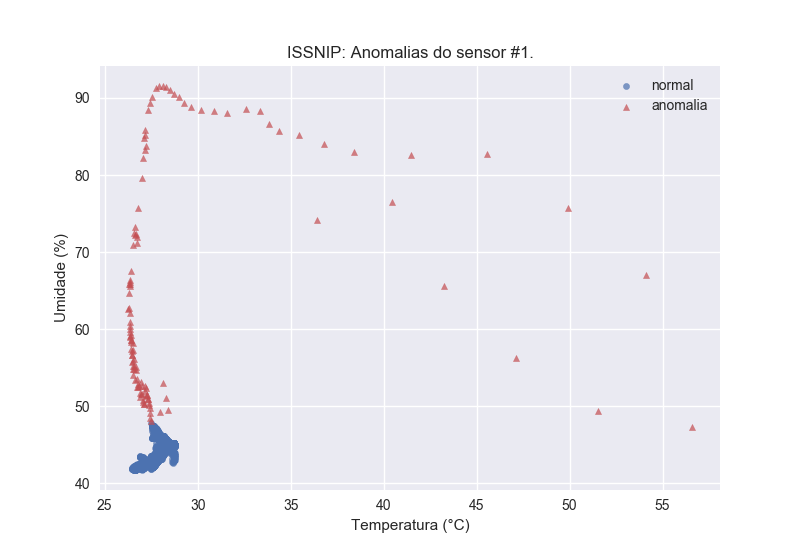
\includegraphics[width=0.68\textwidth]{ISSNIP_1.png}
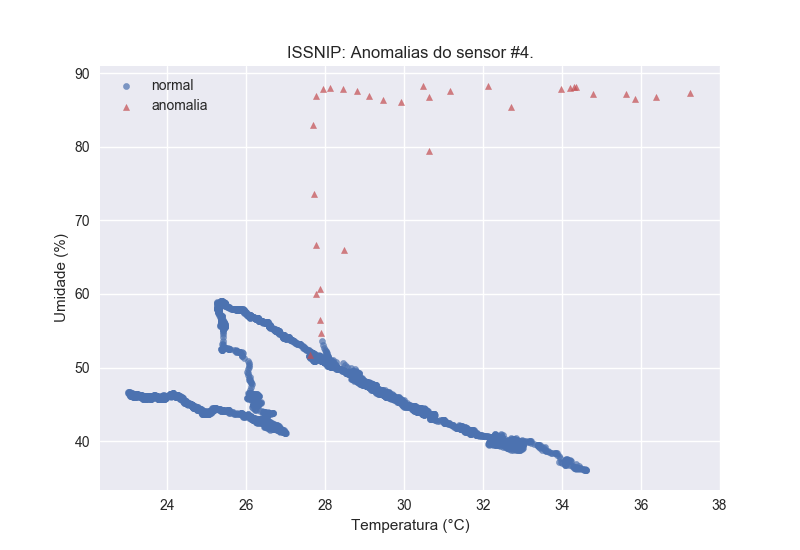
\includegraphics[width=0.68\textwidth]{ISSNIP_4.png}
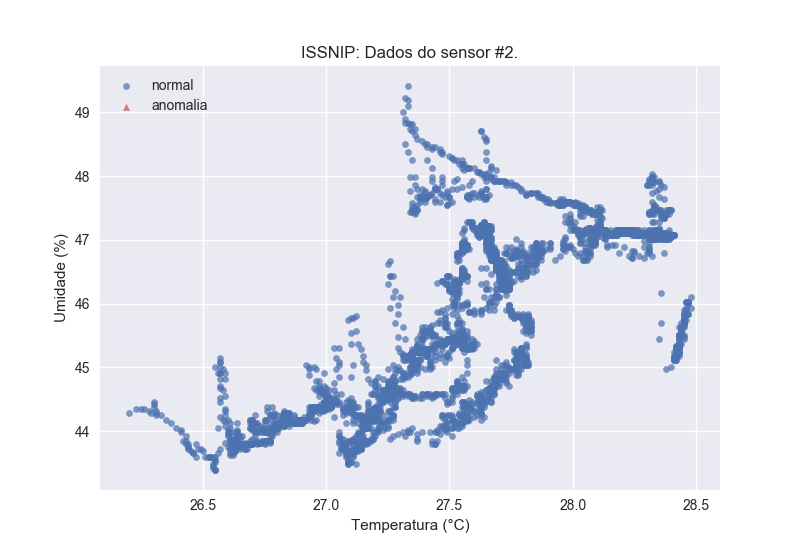
\includegraphics[width=0.68\textwidth]{ISSNIP_2.png}
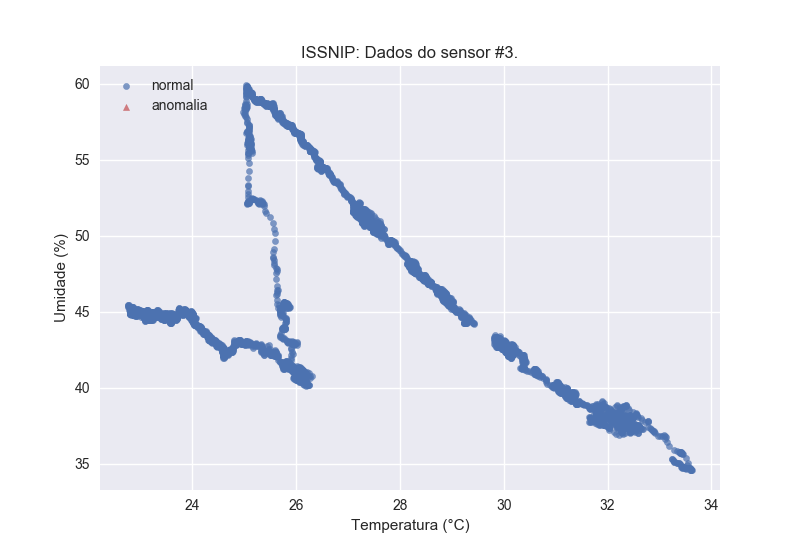
\includegraphics[width=0.68\textwidth]{ISSNIP_3.png}
\caption{Valores de temperatura e umidade do conjunto de dados \textit{ISSNIP}.}
\label{graficos_issnip}
\end{adjustwidth}
\end{figure}

\subsection{\textit{IBRL}: Pré-processamento}

O conjunto de dados \textit{IBRL} não é anotado, isto é, não há informação de quais instâncias dados são normais ou anômalas. Desse modo, seguindo um procedimento semelhante ao apresentado em \cite{DistributedFuzzy2013}, as leituras referentes aos primeiros 18 dias de Março foram extraídas. Nesse período, alguns sensores (\#18, \#19 e \#35) apresentaram mau funcionamento, gerando valores de temperatura longe da região normal, e outros (\#8, \#20) apresentaram algumas leituras anômalas. Após a remoção de valores extremos, os dados foram visualizados e os valores que derivam da região normal foram anotados como anomalias.

A partir da marca temporal das leituras, foram extraídas duas características: \textbf{Hora do Dia} e \textbf{Dia da Semana}. \textbf{Hora do Dia} tem valor 0, se a leitura ocorreu entre 18h e 8h, valor 1, se a leitura ocorreu entre 9h e 12h, ou valor 2, se a leitura ocorreu entre 13h e 17h. \textbf{Dia da Semana} tem valor entre 0 e 6 correspondente aos 7 dias da semana de Domingo a Sábado.

As leituras, características extraídas e a informação de posição dos sensores (atributos \textbf{X} e \textbf{Y}) foram integradas em uma única tabela com 1.378.695 observações, sendo 1.375.656 normais e 3.039 anomalias.~A Figura~\ref{ibrl_normais} mostra os valores de temperatura e umidade de dois sensores do conjunto de dados \textit{IBRL} que apresentam apenas leituras normais como exemplo.~A Figura~\ref{ibrl_anomalos} mostra as observações dos sensores que apresentaram comportamento anômalo. O Apêndice~\ref{app_ibrl} contém exemplos de linhas do conjunto de dados \textit{IBRL}.

\begin{figure}
\begin{adjustwidth}{-1in}{-.8in}
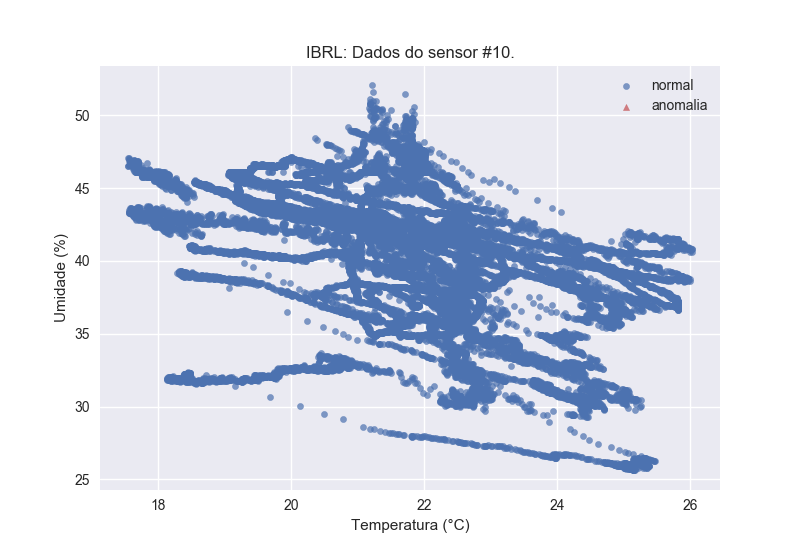
\includegraphics[width=0.68\textwidth]{IBRL_10.png}
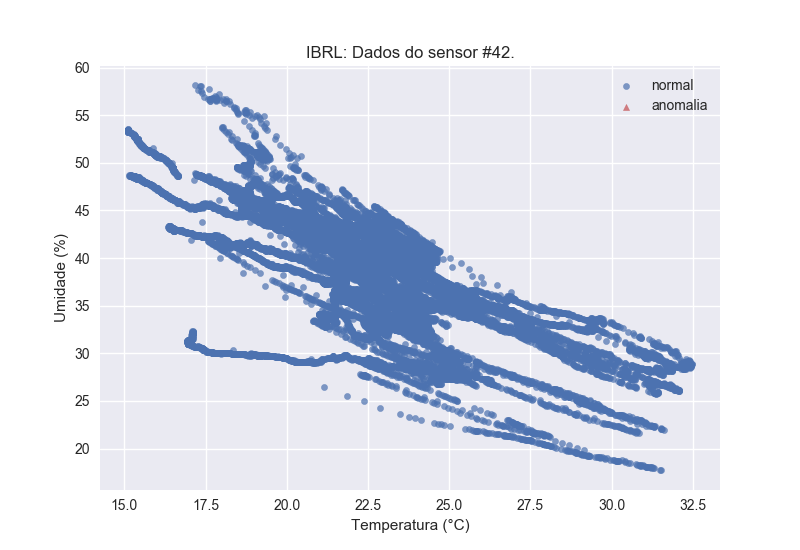
\includegraphics[width=0.68\textwidth]{IBRL_42.png}
\caption{Exemplos de valores de temperatura e umidade normais do conjunto de dados \textit{IBRL}.}
\label{ibrl_normais}
\end{adjustwidth}
\end{figure}

\begin{figure}
\begin{adjustwidth}{-1in}{-.8in}
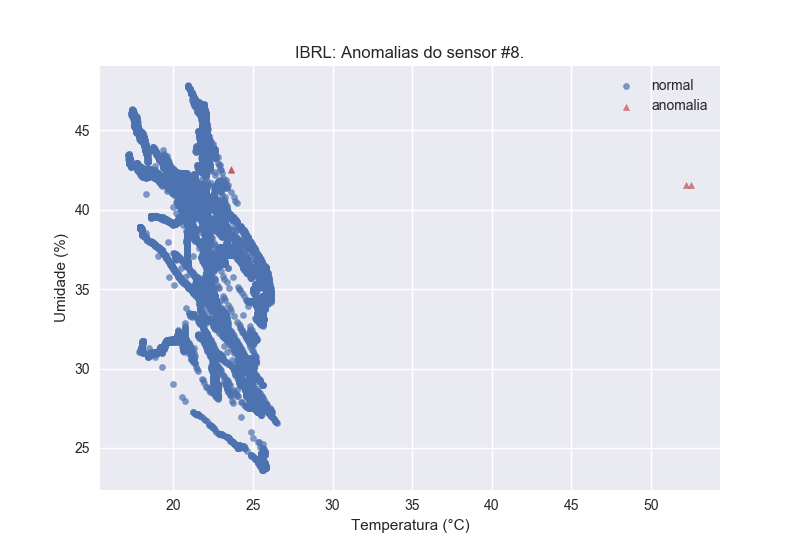
\includegraphics[width=0.68\textwidth]{IBRL_8.png}
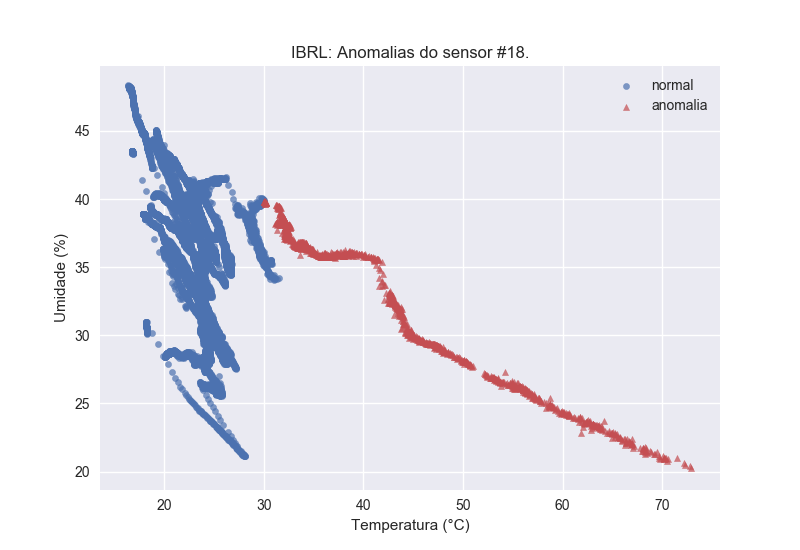
\includegraphics[width=0.68\textwidth]{IBRL_18.png}
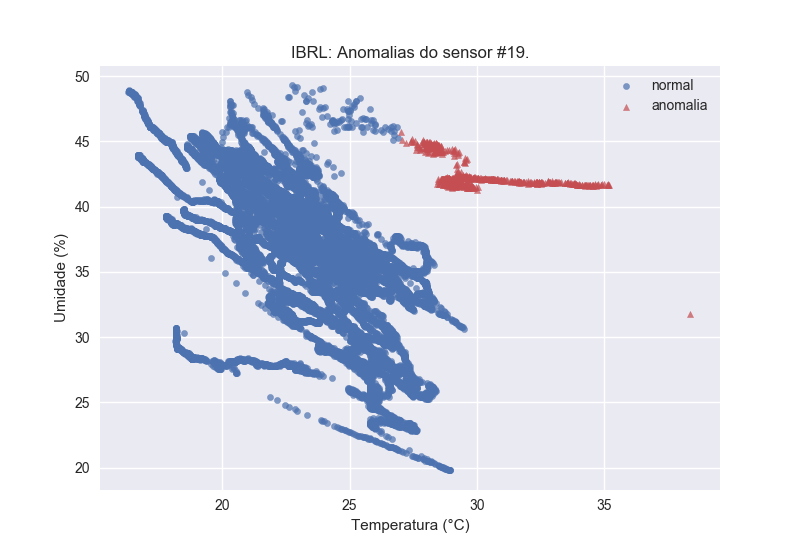
\includegraphics[width=0.68\textwidth]{IBRL_19.png}
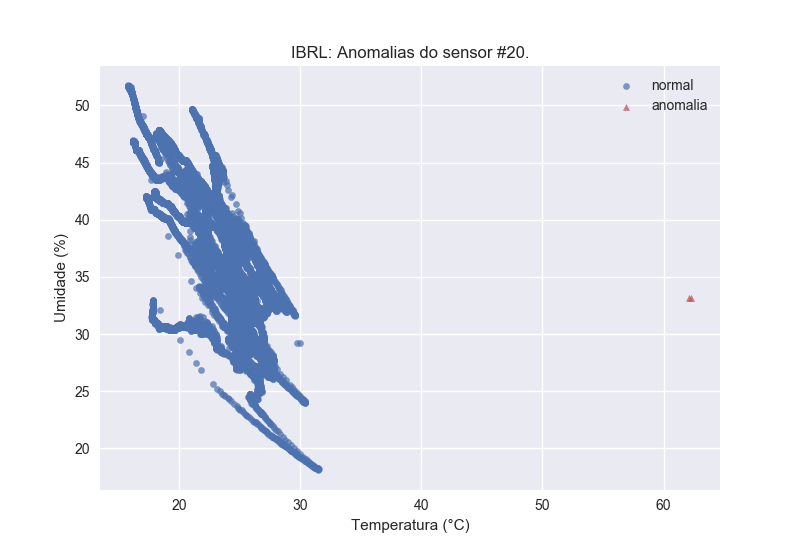
\includegraphics[width=0.68\textwidth]{IBRL_20.png}
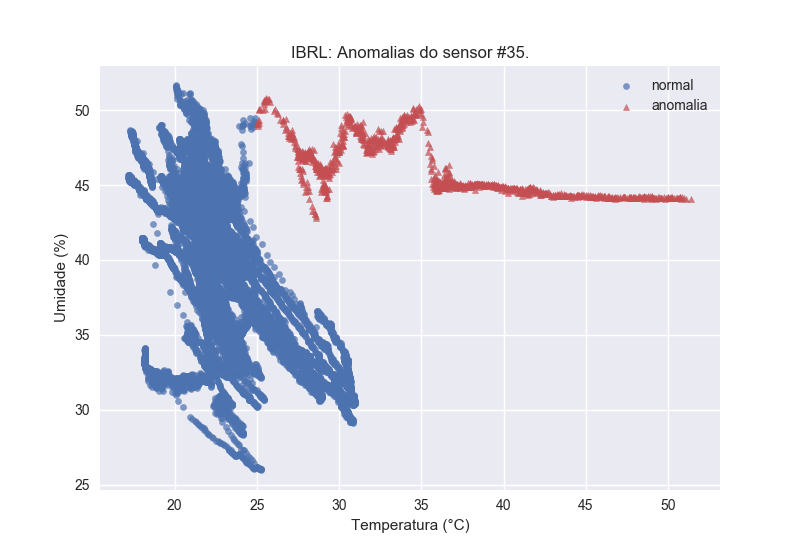
\includegraphics[width=0.68\textwidth]{IBRL_35.png}
\caption{Valores de temperatura e umidade dos sensores que apresentaram leituras anômalas do conjunto de dados \textit{IBRL}.}
\label{ibrl_anomalos}
\end{adjustwidth}
\end{figure}

\subsection{Metodologia}
Os experimentos foram realizados de acordo com um processo de validação cruzada estratificada com 10 iterações (\cite{bootstrap1997}). Para o conjunto de dados \textit{ISSNIP}, cada iteração foi feita com cerca de 16.889 dados normais e 134 dados anômalos de treinamento e cerca de 1.876 dados normais e 15 anomalias de teste. Para o conjunto de dados \textit{IBRL}, cada iteração foi feita com cerca de 1.238.090 dados normais e 2.735 dados anômalos de treinamento e cerca de 137.566 dados normais e 304 dados anômalos de teste. As métricas, definidas na Seção~\ref{metrics}, extraídas dos resultados foram a Precisão, a Revocação, o \textit{F-score} além do número de Verdadeiros Positivos, Verdadeiros Negativos, Falsos Positivos e Falsos Negativos. Os experimentos realizados sobre o conjunto de dados \textit{ISSNIP} foram executados em um computador com processador Intel i7-3770 @ 3.90 GHz e 8GB de memória RAM. Os experimentos realizados sobre o conjunto de dados \textit{IBRL} foram executados em um computador com processador Intel i7-4500U @ 3.0 GHz e 8GB de memória RAM.  

\section{Experimentos Realizados}
Esta Seção descreve os experimentos realizados, explorando a influência dos parâmetros do FDCA, além de tentativas de melhorias no algoritmo.

\subsection{Resultados para o Conjunto de Dados \textit{ISSNIP}}
\label{res_issnip}
Esta seção apresenta os resultados dos experimentos realizados sobre o conjunto de dados \textit{ISSNIP}. A Seção~\ref{issnip_fdca} apresenta os resultados para a execução do sistema sem mudanças. A Seção~\ref{issnip_FA} apresenta os resultados variando o parâmetro $z$ e calculando $z$ dinamicamente. A Seção~\ref{mistura_issnip} apresenta os resultados da segunda mudança, com o agrupamento realizado através da modelagem de mistura Gaussiana.

\subsubsection{Escolha dos Parâmetros do FDCA}
\label{issnip_fdca}
Para cada conjunto de dados, os parâmetros $k$ (Seção~\ref{construcao_sp}) e $c$ (Seção~\ref{sistema_pont}) foram ajustado de modo a buscar o melhor desempenho possível. Para o \textit{ISSNIP}, o parâmetro $k$ foi variado de 1 a 4, buscando a melhoria da capacidade de detecção do componente de detecção contextual. A partir de $k= 3$, não foi observada melhoria significativa, portanto $k = 2$ apresentou os melhores resultados. $c$ foi escolhido, com a ajuda de gráficos de dispersão, de forma a maximizar a revocação do componente de detecção pontual, mantendo o tempo de avaliação da combinação dos componentes abaixo do tempo de execução do componente de detecção contextual. Os parâmetros escolhidos foram $k = 2$ e $c = 0,3$. A adição de mais grupos não resultou em melhoria significativa do desempenho.

\bigskip
\begin{table}[h]
\begin{adjustwidth}{-.5in}{-.5in}
    \caption{Avaliação do FDCA para o conjunto de dados \textit{ISSNIP}}
    \bigskip
    \begin{center}
    \resizebox{\textwidth}{!}{
        \begin{tabular}{|o|c|c|c|c|c|c|c|c|}
          \hline
          \rowcolor{darkorange}
          Modo & Precisão & Revocação & \textit{F-score} & VP & VN & FP & FN & Tempo ($\mu$s)\\
          \hline
          \textit{Pontual} & 0,024 & 0,839 & 0,046 & 12,5 & 1.363,8 & 512,7 &  2,4 & 634\\
          \textit{Contextual} & 0,986 & 0,946 & 0,964 & 14,1 & 1.876,3 & 0,2 & 0,8 & 2.207\\
          FDCA ($z$ = 0,01) & 0,993 & 0,825 & 0,896 & 12,3 & 1.876,4 & 0,1 & 2,6 & 1.269\\
          FDCA (sem $z$) & 0,993 & 0,825 & 0,896 & 12,3 & 1.876,4 & 0,1 & 2,6 & 1.263\\
          \hline
        \end{tabular}}
    \label{av_issnip}
    \end{center}
\end{adjustwidth}
\end{table}

Apenas os dados normais do conjunto de treinamento foram usados para a criação dos perfis de sensores e para a estimação dos Preditores Univariados e Multivariados. Os dados normais e anômalos do conjunto de treinamento foram utilizados para a seleção dos $\epsilon$'s. Por apresentar pouca variância, o atributo \textbf{Localização} foi utilizado apenas durante o agrupamento, sendo ignorado durante a estimação dos Preditores Gaussianos Multivariados. Os parâmetros que apresentaram um melhor desempenho foram $k = 2$ e $c = 0,3$. Os 2 grupos formados pelo algoritmo de agrupamento acabaram por juntar as leituras dos sensores internos em um grupo e as leituras dos sensores externos no outro. A Tabela~\ref{av_issnip} mostra os resultados médios da avaliação do componente de detecção pontual, do componente de detecção contextual, do \textit{framework} completo, com $z = 0,01$ (Seção~\ref{sistema_pont}), e do \textit{framework} sem o fator aleatório, para fins de comparação. Também consta o tempo de execução por instância de dado, em microssegundos.

Observando os resultados da Detecção de Anomalia Pontual e da Detecção de Anomalia Contextual é possível observar o funcionamento do FDCA. A Detecção Contextual possui bom desempenho, apresentando um \textit{F-score} de 0,964, porém a avaliação é muito mais lenta que a Detecção Pontual, levando 3,5 vezes mais tempo. A Detecção Pontual é extremamente imprecisa, mas consegue capturar a maioria das verdadeiras anomalias (aproximadamente 84\%). Os resultados do FDCA mostram como esses dois componentes trabalham juntos para alcançar um bom desempenho, com um \textit{F-score} de 0,896, em um tempo muito menor (57,5\%) do que uma análise puramente contextual.

\subsubsection{Resultados da Avaliação do Fator Aleatório}
\label{issnip_FA}
O FDCA foi executado com os valores de $z =\{0,05;~0,1;~0,25;~0,5\}$. Também foi experimentada uma maneira de calcular $z$ dinamicamente, como detalhado na Seção~\ref{mod_1}. A Tabela~\ref{av_r_issnip} mostra os resultados médios da avaliação para valores de $z = \{0,05;~0,1;~0,25;~0,5\}$ e para o $z$ dinâmico.

\bigskip
\begin{table}[h]
\begin{adjustwidth}{-.5in}{-.5in}
    \caption{Avaliação do fator aleatório do FDCA para o conjunto de dados \textit{ISSNIP}}
    \bigskip
    \begin{center}
    \resizebox{\textwidth}{!}{
        \begin{tabular}{|o|c|c|c|c|c|c|c|c|}
          \hline
          \rowcolor{darkorange}
          Modo & Precisão & Revocação & \textit{F-score} & VP & VN & FP & FN & Tempo ($\mu$s)\\
          \hline
          FDCA ($z$ = 0,05) & 0,993 & 0,826 & 0,899 & 12,3 & 1.876,4 & 0,1 & 2,6 & 1.319\\
          FDCA ($z$ = 0,10) & 0,992 & 0,845 & 0,912 & 12,6 & 1.876,4 & 0,1 & 2,3 & 1.353\\
          FDCA ($z$ = 0,25) & 0,991 & 0,860 & 0,919 & 12,8 & 1.876,4 & 0,1 & 2,1 & 1.519\\
          FDCA ($z$ = 0,50) & 0,987 & 0,905 & 0,942 & 13,5 & 1.876,3 & 0,2 & 1,4 & 1.786\\
          FDCA ($z$ dinâmico) & 0,986 & 0,946 & 0,964 & 14,1 & 1.876,3 & 0,2 & 0,8 & 2.818\\
          \hline
        \end{tabular}}
    \label{av_r_issnip}
    \end{center}
\end{adjustwidth}
\end{table}

É possível concluir que valores baixos para $z$ (até 0,25) tem pouca influência no desempenho do \textit{framework}, apresentando uma melhoria de apenas 2,6\% ao custo de um aumento de 19,7\% no tempo de execução. Mesmo com $z = 0,5$, consegue-se uma melhoria de apenas 5,1\% com um aumento muito maior no tempo de execução (40,7\%). O uso do cálculo dinâmico de $z$ apresenta ótima precisão, igualando-se ao componente de detecção contextual, porém a complexidade do cálculo torna a avaliação muito lenta, tornando seu uso inviável.

\subsubsection{Resultados do Agrupamento por Mistura Gaussiana}
\label{mistura_issnip}
A Tabela~\ref{av_gaussian_issnip} mostra os resultados da avaliação do FDCA com o agrupamento por modelagem de mistura gaussiana. Como pode-se notar, não houve mudanças significativas nos resultados. O tempo de execução do componente de detecção contextual é levemente menor, o que indica que o \textit{framework} demora menos para descobrir a qual perfil de sensor cada leitura pertence.~O restante dos valores semelhantes devem-se ao fato de que o componente de construção de sensores realizou a mesma divisão que o FDCA com agrupamento por \textit{k-means}. 

\begin{table}[h]
\begin{adjustwidth}{-.5in}{-.5in}
    \caption{Avaliação do FDCA com agrupamento por modelagem de mistura Gaussiana para o conjunto de dados \textit{ISSNIP}}
    \bigskip
    \begin{center}
    \resizebox{\textwidth}{!}{
        \begin{tabular}{|o|c|c|c|c|c|c|c|c|}
          \hline
          \rowcolor{darkorange}
          Modo & Precisão & Revocação & \textit{F-score} & VP & VN & FP & FN & Tempo ($\mu$s)\\
          \hline
          \textit{Pontual} & 0,024 & 0,840 & 0,046 & 12,5 &  1.363,5 & 513,0 &  2,4 & 634\\
          \textit{Contextual} & 0,987 & 0,940 & 0,961 & 14,0 & 1.876,3 & 0,2 & 0,9 & 2.026\\
          FDCA ($z$ = 0,01) & 0,992 & 0,820 & 0,896 & 12,2 & 1.876,4 & 0,1 & 2,7 & 1.218\\
          FDCA (sem $z$) & 0,992 & 0,820 & 0,896 & 12,2 & 1.876,4 & 0,1 & 2,7 & 1.214\\
          \hline
        \end{tabular}}
    \label{av_gaussian_issnip}
    \end{center}
\end{adjustwidth}
\end{table}

\subsection{Resultados para o Conjunto de Dados \textit{IBRL}}
\label{res_ibrl}
Esta seção apresenta os resultados dos experimentos realizados sobre o conjunto de dados \textit{IBRL}. A Seção~\ref{ibrl_fdca} apresenta os resultados para a execução do sistema sem mudanças. A Seção~\ref{ibrl_FA} apresenta os resultados variando o parâmetro $z$ e calculando $z$ dinamicamente. A Seção~\ref{mistura_ibrl} apresenta os resultados da segunda mudança, com o agrupamento realizado através da modelagem de mistura Gaussiana.

\subsubsection{Escolha dos Parâmetros do FDCA}
\label{ibrl_fdca}
Para o \textit{IBRL}, $k$ foi escolhido com base em \cite{Ellipsoids2009}, que realiza avaliações sobre o mesmo conjunto de dados. O autor escolhe $k = 4$ para um procedimento de agrupamento com base no gráfico dos autovalores do conjunto. Novamente, $c$ foi escolhido, também com a ajuda de gráficos de dispersão, de modo capturar a maioria das anomalias verdadeiras, mantendo um tempo de execução satisfatório. Os parâmetros escolhidos foram $k = 4$ e $c = 0,005$.

Assim como no caso do \textit{ISSNIP}, apenas os dados normais do conjunto de treinamento foram usados para a a construção dos perfis de sensores e definição dos parâmetros do Preditores Univariados e Multivariados. As anomalias do conjunto de treinamento foram incluídas durante a seleção dos $\epsilon$'s. O atributo \textbf{Hora do Dia} apresentou pouca variância e foi considerado apenas durante o agrupamento, sendo ignorado durante o cálculo dos parâmetros dos Preditores Gaussianos Multivariados. Os parâmetros escolhidos foram $k = 4$ e $c = 0,005$. Não houve padrão observado no agrupamento resultante da criação de perfis de sensores. A Tabela~\ref{av_ibrl} apresenta os resultados médios para os diversos componentes do \textit{framework}, além de resultados para a execução sem o fator aleatório. O tempo, em microssegundos, é a duração média da avaliação de uma instância de dado.

\bigskip
\begin{table}[h]
\begin{adjustwidth}{-.5in}{-.5in}
    \caption{Avaliação do FDCA para o conjunto de dados \textit{IBRL}}
    \bigskip
    \begin{center}
    \resizebox{\textwidth}{!}{
        \begin{tabular}{|o|c|c|c|c|c|c|c|c|}
          \hline
          \rowcolor{darkorange}
          Modo & Precisão & Revocação & \textit{F-score} & VP & VN & FP & FN & Tempo ($\mu$s)\\
          \hline
          \textit{Pontual} & 0,035 & 0,999 & 0,068 & 303,7 & 129.223,8 & 8.341,8 & 0,2 & 449\\
          \textit{Contextual} & 0,998 & 0,788 & 0,881 & 239,6 & 137.565,2 & 0,4 & 64,3 & 1.324\\
          FDCA ($z$ = 0,01) & 0,998 & 0,788 & 0,881 & 239,6 & 137.565,2 & 0,4 & 64,3 & 545\\
          FDCA (sem $z$) & 0,998 & 0,788 & 0,881 & 239,6 & 137.565,2 & 0,4 & 64,3 & 540\\
          \hline
        \end{tabular}}
    \label{av_ibrl}
    \end{center}
\end{adjustwidth}
\end{table}

\bigskip
\bigskip
Pela Tabela~\ref{av_ibrl} pode-se concluir que o FDCA apresentou um ótimo desempenho, capturando 82\% das instâncias anômalas e classificando-as com 99,9\% de precisão, em média. Novamente, pode-se notar que o componente de detecção contextual, apesar de preciso, é muito mais lento que o componente de detecção pontual, demorando 3 vezes mais tempo para avaliar uma instância de dado. Os dois componentes operando em conjunto no FDCA alcançam o mesmo \textit{F-score} do componente de detecção contextual em apenas 42\% do tempo.

\subsubsection{Resultados da Avaliação do Fator Aleatório}
\label{ibrl_FA}
Para o conjunto de dados \textit{IBRL}, foi avaliada apenas a influência do cálculo dinâmico de $z$. Como pode ser observado na Tabela~\ref{av_z_ibrl}, o uso do $z$ dinâmico não modificou a capacidade de detecção do \textit{framework}, além de tornar a avaliação muito mais lenta.

\bigskip
\begin{table}[h]
\begin{adjustwidth}{-.5in}{-.5in}
    \caption{Avaliação do fator aleatório do FDCA para o conjunto de dados \textit{IBRL}}
    \bigskip
    \begin{center}
    \resizebox{\textwidth}{!}{
        \begin{tabular}{|o|c|c|c|c|c|c|c|c|}
          \hline
          \rowcolor{darkorange}
          Modo & Precisão & Revocação & \textit{F-score} & VP & VN & FP & FN & Tempo ($\mu$s)\\
          \hline
          FDCA ($z$ dinâmico) & 0,998 & 0,788 & 0,881 & 239,6 & 137.565,2 & 0,4 & 64,3 & 1.724\\
          \hline
        \end{tabular}}
    \label{av_z_ibrl}
    \end{center}
\end{adjustwidth}
\end{table}

\subsubsection{Resultados do Agrupamento por Mistura Gaussiana}
\label{mistura_ibrl}
Como pode ser observado na Tabela~\ref{av_gaussian_ibrl}, a utilização do agrupamento do modelagem de mistura gaussiana melhorou o \textit{F-score} em 3,6\%, o que significa que o algoritmo conseguiu modelar melhor a distribuição dos dados do que o agrupamento por \textit{k-means}. Essa versão do FDCA conseguiu capturar 5\% anomalias verdadeiras a mais do que a versão sem a mudança.

\bigskip
\begin{table}[h]
\begin{adjustwidth}{-.5in}{-.5in}
    \caption{Avaliação do FDCA com agrupamento por modelagem de mistura Gaussiana para o conjunto de dados \textit{IBRL}}
    \bigskip
    \begin{center}
    \resizebox{\textwidth}{!}{
        \begin{tabular}{|o|c|c|c|c|c|c|c|c|}
          \hline
          \rowcolor{darkorange}
          Modo & Precisão & Revocação & \textit{F-score} & VP & VN & FP & FN & Tempo ($\mu$s)\\
          \hline
          \textit{Pontual} & 0,035 & 0,999 & 0,068 & 303,7 & 129.224,9 & 8.340,7 & 0,2 & 441\\
          \textit{Contextual} & 0,998 & \textbf{0,841} & \textbf{0,913} & 255,7 & 137.565,0 & 0,6 & 48,2 & 1.331\\
          FDCA ($z$ = 0,01) & 0,998 & \textbf{0,841} & \textbf{0,913} & 255,7 & 137.565,0 & 0,6 & 48,2 & 534\\
          FDCA (sem $z$) & 0,998 & \textbf{0,841} & \textbf{0,913} & 255,7 & 137.565,0 & 0,6 & 48,2 & 526\\
          \hline
        \end{tabular}}
    \label{av_gaussian_ibrl}
    \end{center}
\end{adjustwidth}
\end{table}

\section{Análise Geral dos Resultados}
É possível concluir que o FDCA detectou as anomalias com desempenho satisfatório nos dois conjuntos de dados apresentados. O tempo de avaliação de cada instância de dados se mostrou satisfatório e indica que o \textit{framework} é adequado para a detecção de anomalias em redes de sensores no contexto de \textit{Big Data}, onde centenas de milhares de sensores podem estar enviando dados para uma central a cada segundo.

Um ponto fraco do \textit{framework} é que sua eficiência depende do quão bem os Preditores modelam a distribuição dos dados. Pode-se notar que o \textit{framework} apresentou um \textit{F-score} levemente melhor avaliando o conjunto de dados \textit{IBRL} do que avaliando o conjunto \textit{ISSNIP}. Isso ocorre, em parte, porque a distribuição do \textit{IBRL} se aproxima mais de uma distribuição normal do que a distribuição do \textit{ISSNIP}.

Das mudanças propostas, a utilização da Equação~\ref{dinamic_z} para o cálculo dinâmico de $z$ não modificou a capacidade de detecção do algoritmo, além de aumentar demasiadamente o tempo de execução. A segunda mudança, o agrupamento por modelagem de mistura gaussiana, apresentou uma leve melhoria (de um \textit{F-score} de 0,881 para um \textit{F-score} de 0,913) na avaliação do conjunto de dados \textit{IBRL}.

\chapter{Conclusões}
\label{conclusao}
O trabalho intitulado \textit{Contextual Anomaly Detection for Big Sensor Data} \cite{ContextualMichael2014} apresenta um \textit{framework} para a detecção de anomalias em dados provenientes de redes de sensores. O algoritmo apresentado tem como objetivo realizar a detecção de anomalias utilizando informações contextuais resultando em um sistema rápido, escalável, apropriado para o contexto de \textit{Big Data}, onde os dados são gerados rapidamente, podem originar de centenas de milhares de fontes e necessitam de avaliação em tempo real ou quase real.

O sistema proposto, denominado FDCA, foi implementado em \textit{Python} e avaliado em dois conjuntos de dados, o \textit{ISSNIP} e o \textit{IBRL}. Também foram analisadas possibilidades de melhorias no \textit{framework}, calculando o parâmetro $z$ (Seção~\ref{sistema_pont}) dinamicamente e realizando o agrupamento durante a criação de perfis de sensores através de modelagem de mistura gaussiana.

O FDCA apresentou bons resultados, apresentando um \textit{F-score} de cerca de 0,9 para os dois conjuntos de dados.~Das modificações propostas, apenas a utilização do agrupamento por modelagem de mistura gaussiana resultou em uma pequena melhoria da capacidade de detecção do \textit{framework}.

Futuros trabalhos podem ser realizados de forma a explorar a viabilidade de uma maneira eficiente de mandar amostras para o detector contextual apesar da normalidade perante o detector pontual (fator aleatório). Também pode-se explorar como generalizar o \textit{framework} para outras distribuições de dados, visto que é um dos pontos fracos dessa abordagem.

\bibliographystyle{abntex2-alf}
\bibliography{biblio}

\appendix
\chapter{Exemplos do Conjunto de Dados \textit{IBRL}}
\label{app_ibrl}

\begin{table}[h]
    \begin{adjustwidth}{-0.7in}{-0.7in}
    \begin{center}
    \resizebox{1.15\textwidth}{!}{
    \begin{tabular}{ccccccccccccc}
    \hline
    Data & Hora & Epoch & ID & Temperatura & Umidade & Luz & Tensão & X & Y & H & S & A \\
    \hline
    2004-03-01 & 0:01:57 & 5648 & 1 & 18.4498 & 43.1191 & 43.24 & 2.67532 & 21.5 & 23 & 0 & 0 & 0 \\
    2004-03-01 & 0:02:50 & 5650 & 1 & 18.44 & 43.0858 & 43.24 & 2.66332 & 21.5 & 23 & 0 & 0 & 0 \\
    2004-03-01 & 0:04:27 & 5653 & 1 & 18.44 & 43.1191 & 43.24 & 2.65143 & 21.5 & 23 & 0 & 0 & 0 \\
    2004-03-01 & 0:05:28 & 5655 & 1 & 18.4498 & 43.0524 & 43.24 & 2.65143 & 21.5 & 23 & 0 & 0 & 0 \\
    2004-03-01 & 0:05:50 & 5656 & 1 & 18.4302 & 43.1525 & 43.24 & 2.66332 & 21.5 & 23 & 0 & 0 & 0 \\
    2004-03-01 & 0:09:27 & 5663 & 1 & 18.44 & 43.1858 & 43.24 & 2.66332 & 21.5 & 23 & 0 & 0 & 0 \\
    2004-03-01 & 0:09:51 & 5664 & 1 & 18.4302 & 43.2525 & 43.24 & 2.65143 & 21.5 & 23 & 0 & 0 & 0 \\
    2004-03-01 & 0:10:21 & 5665 & 1 & 18.4302 & 43.2525 & 43.24 & 2.65143 & 21.5 & 23 & 0 & 0 & 0 \\
    2004-03-01 & 0:13:51 & 5672 & 1 & 18.4302 & 43.2858 & 43.24 & 2.67532 & 21.5 & 23 & 0 & 0 & 0 \\
    2004-03-01 & 0:18:26 & 5681 & 1 & 18.391 & 43.3858 & 43.24 & 2.66332 & 21.5 & 23 & 0 & 0 & 0 \\
    2004-03-01 & 0:18:51 & 5682 & 1 & 18.391 & 43.3525 & 43.24 & 2.65143 & 21.5 & 23 & 0 & 0 & 0 \\
    2004-03-01 & 0:19:56 & 5684 & 1 & 18.391 & 43.3525 & 43.24 & 2.65143 & 21.5 & 23 & 0 & 0 & 0 \\
    2004-03-01 & 0:20:51 & 5686 & 1 & 18.391 & 43.2191 & 43.24 & 2.65143 & 21.5 & 23 & 0 & 0 & 0 \\
    2004-03-01 & 0:22:21 & 5689 & 1 & 18.3812 & 43.2858 & 43.24 & 2.66332 & 21.5 & 23 & 0 & 0 & 0 \\
    2004-03-01 & 0:22:51 & 5690 & 1 & 18.391 & 43.3191 & 43.24 & 2.66332 & 21.5 & 23 & 0 & 0 & 0 \\
    2004-03-18 & 23:32:33 & 57428 & 35 & 48.5946 & 44.2168 & 172.96 & 2.31097 & 24.5 & 27 & 0 & 3 & 1 \\
    2004-03-18 & 23:33:48 & 57431 & 35 & 48.3202 & 44.2168 & 172.96 & 2.30202 & 24.5 & 27 & 0 & 3 & 1 \\
    2004-03-18 & 23:34:17 & 57432 & 35 & 48.9474 & 44.2168 & 172.96 & 2.30202 & 24.5 & 27 & 0 & 3 & 1 \\
    2004-03-18 & 23:34:48 & 57433 & 35 & 48.771 & 44.2499 & 172.96 & 2.30202 & 24.5 & 27 & 0 & 3 & 1 \\
    2004-03-18 & 23:35:22 & 57434 & 35 & 48.918 & 44.2499 & 172.96 & 2.30202 & 24.5 & 27 & 0 & 3 & 1 \\
    \hline
    \end{tabular}}
    \end{center}
    \end{adjustwidth}
    \bigskip
    \legend{Os atributos \textbf{Hora do Dia}, \textbf{Dia da Semana} e \textbf{Anotação} foram abreviados para \textbf{H}, \textbf{S} e \textbf{A}, respectivamente}
\end{table}

\chapter{Exemplos do Conjunto de Dados \textit{ISSNIP}}
\label{app_issnip}

\begin{table}[h]
\begin{center}
    \begin{tabular}{cccccc}
    \hline
    Leitura\# & ID & Umidade & Temperatura & Anotação & Localização \\
    \hline
    1 & 1 & 45.93 & 27.97 & 0 & 1 \\
    2 & 1 & 45.9 & 27.95 & 0 & 1 \\
    3 & 1 & 45.9 & 27.96 & 0 & 1 \\
    4 & 1 & 45.93 & 27.95 & 0 & 1 \\
    5 & 1 & 45.93 & 27.97 & 0 & 1 \\
    6 & 1 & 45.9 & 27.98 & 0 & 1 \\
    7 & 1 & 45.9 & 27.95 & 0 & 1 \\
    8 & 1 & 45.97 & 27.94 & 0 & 1 \\
    9 & 1 & 46 & 27.92 & 0 & 1 \\
    10 & 1 & 46.1 & 27.92 & 0 & 1 \\
    11 & 1 & 46.1 & 27.9 & 0 & 1 \\
    5026 & 4 & 46.1 & 23.08 & 0 & 0 \\
    5027 & 4 & 46.1 & 23.07 & 0 & 0 \\
    5028 & 4 & 46.1 & 23.07 & 0 & 0 \\
    5029 & 4 & 46.13 & 23.06 & 0 & 0 \\
    5030 & 4 & 46.23 & 23.04 & 0 & 0 \\
    2443 & 1 & 50.8 & 27.05 & 1 & 1 \\
    2444 & 1 & 50.51 & 27.07 & 1 & 1 \\
    2445 & 1 & 50.26 & 27.1 & 1 & 1 \\
    2446 & 1 & 50.35 & 27.13 & 1 & 1 \\
    2447 & 1 & 51.92 & 27.16 & 1 & 1 \\
    \hline
    \end{tabular}
    \end{center}
    \bigskip

\end{table}


\end{document}
